\documentclass[12pt,a4paper]{report}
\usepackage[utf8]{inputenc}
\usepackage{amsmath}
\usepackage{amsfonts}
\usepackage{amssymb}
\usepackage{color}
\usepackage[bb=boondox]{mathalfa}
\usepackage{graphicx}
\usepackage{placeins}
\usepackage{mathtools}
\usepackage[nottoc]{tocbibind}
\usepackage{pdfpages}
\usepackage{url}

%\DeclareMathAlphabet{\mathbbold}{U}{bbold}{m}{n}

%\newcommand{\draft}[1]{\textcolor{red}{#1}}
\newcommand{\draft}[1]{\textcolor{magenta}{\underline{#1}}}
%\newcommand{\draft}[1]{#1}
\DeclareMathOperator\erf{erf}
\DeclareMathOperator\erfc{erfc}

\author{Aleksei Iupinov}
\title{Particle Mesh Ewald on a GPU}

\begin{document}
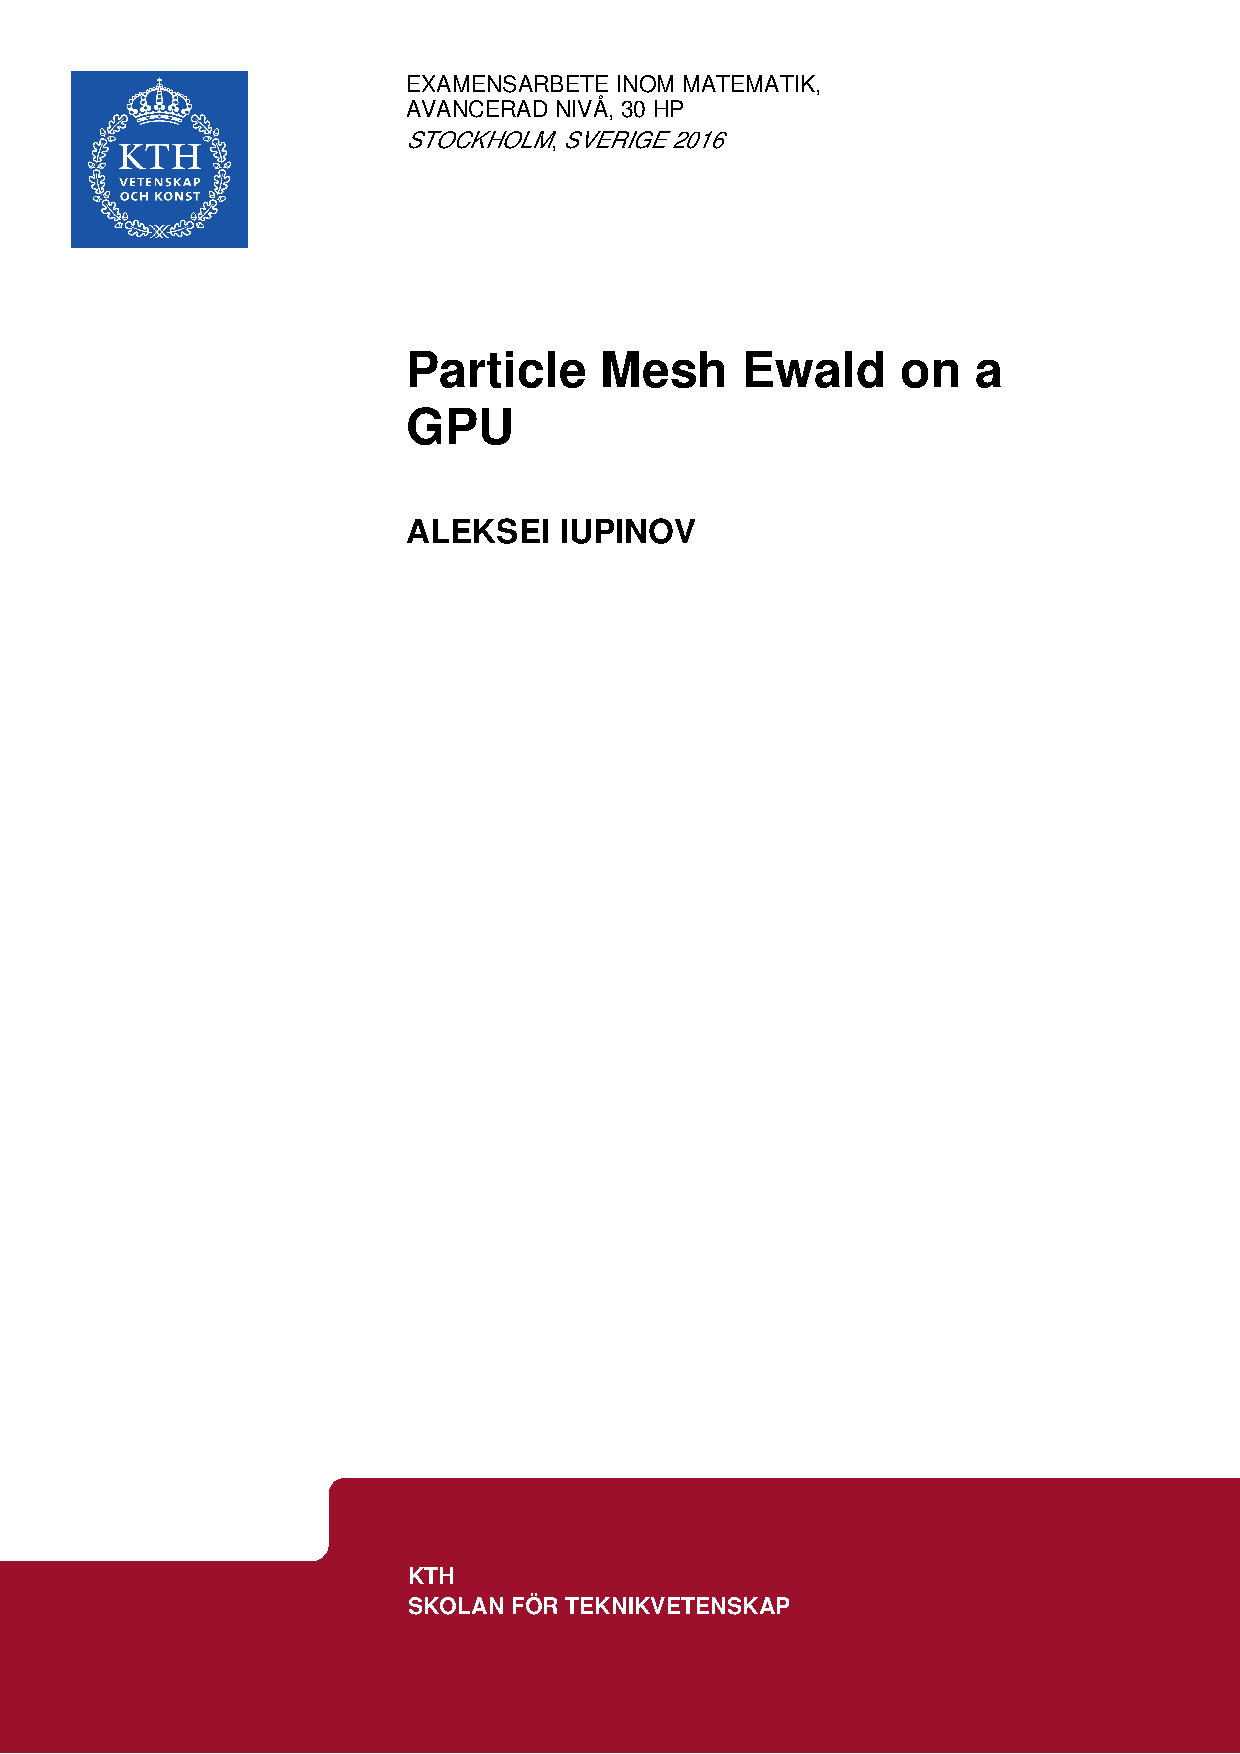
\includepdf[pages={1-2}]{pics/cover.pdf}

\begin{abstract}

The Particle Mesh Ewald (PME) method is used for efficient long-range electrostatic calculations in molecular dynamics (MD).
 
In this project, PME is implemented for a single GPU alongside the existing CPU implementation, using the code base of an open source MD software GROMACS and NVIDIA CUDA toolkit. The performance of the PME GPU implementation is then studied. 

The motivation for the project is examining the PME algorithm's parallelism, and its potential benefit for performance scalability of MD simulations on various hardware. 

%\draft{Should be translated to Swedish as well.}

\end{abstract}
\newpage

\tableofcontents
\newpage


\iffalse
In molecular simulations most of the time in the computation is spent on calculating electrostatic interactions between pairs of atoms. The Coulomb interactions between charges decay as 1/r (where r is the distance between particles). This decay is very slow and means that one can not simply neglect interactions beyond a certain distance. Molecular systems are often treated with periodic boundary conditions, which leads to an infinite number of pair interactions. To make the force calculating tractable, the forces are split into a short-range, steep component and a long-range, smooth component. The most efficient way to calculate the forces is the so called Particle-Mesh-Ewald (PME) method (*). The short-range component is calculated directly by looping over pairs at short distance. The long-range component is obtained by spreading charged to a grid, determining the 3D-FFT of the charge grid, multiplying with the influence function in Fourier space, back FFT, gathering the particle forces from the grid. Achieving maximal performance on these components is critical for good performance of molecular simulations in general and in particular of the GROMACS package, which will be used in this project. Apart from the multiplication in the Fourier space, which is straightforward to vectorize, designing good algorithms for the other components is non-trivial. On the CPU most simulation packages have converged to the same approach. But here most components can not take advantage of SIMD instructions of width 8 (AVX) or more (AVX512). As of a few years GPUs are becoming increasingly for running molecular simulations. This can be done in two ways, either run (nearly) everything on the GPU, or run a part of the compute tasks on the GPU. GROMACS takes the latter approach. Currently we have only the particle-pair interactions running on the GPU. But moving part or all of the PME mesh calculation could benefit performance significantly on current hardware. Some future hardware might have very weak CPUs compared to the GPUs and nearly everything will have to run on the GPU. The results of this project will directly benefit thousands of GROMACS users world-wide. The future benefit will be even higher, because we expect supercomputers to also get relatively more GPU/accelerator power that we can only benefit from by running PME on the GPUs.

Project tasks

We already have basic (slow) versions of the different PME mesh components working on the GPU in CUDA. The main task it to find out which algorithms will work best for each component. The parts where this is more unclear are the charge spreading and the force gathering. Here there are many options for grouping computations, task division over threads and data layout. Especially for the charge spreading there are different algorithmic options, such as transforming spreading to charge-gathering to grid points. For the 3D-FFT there are GPU libraries available, here it is probably mostly a matter of finding the best parameters. A second, related task is to decide which tasks to run together in one kernel and which to separate. Also related is the decision of which tasks to run on the CPU and the GPU in the case of running PME in a mixed CPU-GPU setup. Parallelization over multiple GPUs and/or MPI ranks is mostly taken care of at the higher level and does not need to be considered in this project. (If there is time and interest left, one could look at how to do the 3D-FFT on multiple GPUs with direct GPU-GPU communication.) Since most of the setup work is already done, this project can focus on the choice, implementation, benchmarking and tuning of different algorithms. We have a numerical analysis and algorithm expert (Berk Hess) and CUDA algorithm expert (Szilard Pall) in the group. In addition we have access to our own technical support engineer at Nvidia. He has already looked into our preliminary code. Although there are other molecular simulation codes out there that run PME on the GPU (which we can take inspiration from), up till now nothing has been published on this topic, so this work could lead to a scientific publication.


\fi





\newpage
\chapter{Introduction}

In this chapter the project domain, objective and scope are outlined.

\section{Domain}

High performance is important in molecular dynamics (MD) simulations, as they are commonly used for modelling complex organic molecules and structures on various scales. System sizes may vary from hundreds to millions particles. Time scales may vary up to trillions of time steps - a single time step is usually on the order of femtoseconds while the duration of processes being modelled might range from nanoseconds to milliseconds.

The main computational effort of a MD simulation time step is the calculation of the electrostatic forces, which, if implemented naively (each to each), would scale as the square of the number of particles $O(N^2)$.

Particle Mesh Ewald (PME) is a long-range interactions computation algorithm for periodic systems. It is based on the Ewald summation, first described in 1921 \cite{ewald}. Originally it was used for the ionic crystals' energy calculation. The method requires periodic boundary conditions and charge neutrality of the molecular system in order to accurately calculate the total Coulombic interaction. 

The idea of the PME method in short is as follows: all the long-range energy contributions (usually selected by a splitting function) are calculated in Fourier space, where they converge faster than the the real-space $\frac{1}{\lvert r\rvert}$ dependency in direct summation. The computational effort of a long-range component in PME is $ O(N\cdot\log(N))$. The method is described in more detail in the next chapter.
 
\section{Objective} 
 
In this project, the PME method is implemented in a highly-parallel code running on a GPU, using NVIDIA CUDA toolkit, as a part of an open-source molecular dynamics software package GROMACS. 
% \cite{gromacs50}}.
Achieving good performance of PME on GPU is important for good performance of molecular simulations in general and in particular for the GROMACS package. As of a few years GPUs are becoming increasingly important for running molecular simulations. The need for a strong scaling (as partially provided by thousands of cores on a typical GPU) and the current CPU performance bottleneck dictate the need for parallel GPU implementations of existing algorithms.

There are two approaches to the GPU programming, either run (nearly) everything on the GPU, or run only a part of the compute tasks on the GPU for better system utilization. GROMACS takes the latter approach. Currently only the non-bonded short-range particle pair interactions are being computed on the GPU. Moving part or all of the PME calculation onto the GPU could benefit performance significantly on current hardware. Some future hardware might have very weak CPUs compared to the GPUs and nearly everything will have to run on the GPU. The results of this project will directly benefit thousands of GROMACS users world-wide. The future benefit will be even higher, because supercomputers are also expected to also get relatively more GPU/accelerator power.

\section{Scope} \label{chapter_scope}

The scope of this project is to implement PME on GPU in C++/CUDA C within GROMACS code base.
There are several design constraints here:
\begin{itemize}
\item The method is implemented using NVIDIA CUDA toolkit (only for NVIDIA hardware). The reasons for choosing CUDA over OpenCL, a viable alternative standard, are practical - NVIDIA is currently the main GPU hardware producer; the NVIDIA CUDA library generally gives better performance than NVIDIA OpenCL implementation; and above all that, once the prototype is complete, it is not difficult to reimplement the same algorithms in OpenCL, as the core OpenCL C/CUDA C language concepts are similar. GROMACS users would much more benefit from the CUDA PME implementation.
\item The method is implemented for a single PME simulation process working with a single GPU. GROMACS employs various parallelization techniques for better scaling, including domain decomposition algorithms, where parts of the domain are treated by different processes within the same simulation (read more about it in the section \ref{chapter:DD}). The existing CPU PME implementation supports multi-process computation as well. 
However, a prospect of multi-GPU PME implementation is raising additional concerns, such as minimisation of the communication costs between GPUs, domain decomposition algorithms, and load balancing. While this should certainly be considered during future developments of PME GPU, a PME implementation for a single GPU should provide a foundation for that, highlighting the weak and strong points of the implementation and its scalability. 
Also note that the PME amounts only to a part of the total computation, while the other component (short-rage work, see section \ref{rangeimpl}) is already scalable over multiple processes/GPUs in GROMACS. Therefore, having PME computation sped up on a single process with the use of a dedicated GPU can already be beneficial for small-scale simulations running on a single machine with one or several GPUs.
\item The room for a scalable multi-GPU implementation is left in the implementation. The major part of the communication latency introduced with the multi-node scaling is caused by the the 3D FFT stages of the algorithm. For this reason, the PME GPU implementation has to provide an option to perform the FFT computation on CPU instead of GPU (more about it in the section \ref{FFTimpl}).

\end{itemize}
\iffalse

In molecular simulations most of the time in the computation is spent on calculating electrostatic interactions between pairs of atoms. The Coulomb interactions between charges decay as $\frac{1}{\lvert r \rvert}$ (where $r$ is the distance between particles). This decay is very slow and means that one can not simply neglect interactions beyond a certain distance.

 Molecular systems are often treated with periodic boundary conditions, which leads to an infinite number of pair interactions. To make the force calculating tractable, the forces are split into a short-range, steep component and a long-range, smooth component. The most efficient way to calculate the long-range forces is the so called Particle Mesh Ewald (PME) method. The short-range component is calculated directly by looping over pairs at short distance. 
 
The long-range component is obtained by spreading charged to a grid, determining the 3D-FFT of the charge grid, multiplying with the influence function in Fourier space, back FFT, gathering the particle forces from the grid. 




The input data for PME is particle coordinates within unit cell, and their charges.  The output data is forces acting on each particles, the reciprocal energy and the virial of the system.

 Direct category is then calculated just like before, in the "naive" way, while non-direct is transformed into complex Fourier space, DERPed, transformed back (details in the next session).
In the current version of Gromacs (5.1) there is support different architecture-depended ILP (AVX, SIMD,... ), TLP (OpenMP) as well as CUDA, OpenCL. As the direct particle-to particle interaction is so significant for MD simulation performance, this part has all these SImd implementations in GROMACS, and is the only part that has the GPU codepathwaythingie.
\fi

\newpage

\chapter{The PME method}
In this chapter, the Ewald summation and the smooth PME approach are described briefly.

\iffalse

\draft{
The reciprocal Ewald sum is the solution to Poisson’s equation in periodic boundary conditions, with Gaussian charge densities as sources. 
}
\fi

\section{Ewald summation} \label{sec_ewald}
In an electrostatic calculation with periodic boundary conditions, one first assumes that the system is contained in a so called unit cell $U$. Let $U$ be defined by the edge vectors $\bold{a}_1, \bold{a}_2, \bold{a}_3$, which are not necessarily orthogonal. We can also define for later use conjugate reciprocal vectors $\bold{a}_1^*, \bold{a}_2^*, \bold{a}_3^*$ such that $\bold{a}_i^* \bold{a}_j = \delta_{ij}$ (Kronecker delta).
 Let there be $N$ point charges $q_1, \dotsc, q_N$ with positions $\bold{r}_1, \dotsc, \bold{r}_N$ within $U$ satisfying charge neutrality:  $\sum\limits_{i=1}^N q_i=0$. We can define fractional coordinates of charge $q_j$ by $s_{kj} = \bold{a}_k^* \cdot \bold{r}_j$, where $k = 1, 2, 3$. 
\\
The charges interact according to Coulomb’s law with periodic boundary conditions. Thus a point charge $q_i$ at position $\bold{r}_i$ interacts with
other charges $q_j$, $j \neq i$ at positions $\bold{r}_j$ as well as with all of
their periodic images at positions $\bold{r}_j + n_1 \bold{a}_1  + n_2 \bold{a}_2  + n_3 \bold{a}_3$ for
all $n_1, n_2 , n_3 \in \mathbb{Z}$. It also interacts with its own periodic
images at $\bold{r}_i + n_1 \bold{a}_1  + n_2 \bold{a}_2  + n_3 \bold{a}_3$, only that  $\bold{n} = (n_1, n_2, n_3)^T \neq \mathbb{0}$ to exclude the original. 

An electrostatic energy of the unit cell can be written:

\begin{equation} \label{eq:ewald}
E(\bold{r}_1, \dotsc, \bold{r}_N) = \frac{1}{2} \sum\limits_{\bold{n} \in \mathbb{Z}^3}^* \sum_{i=1}^N \sum\limits_{j=1}^N \frac{q_i q_j}{\lvert\bold{r}_i - \bold{r}_j + \bold{n} \rvert}
\end{equation}
The asterisk on the outer sum signifies that the contributions with zero denominator ($i =j$ and $\bold{n} = \mathbb{0}$) are omitted.

The outer infinite series in \eqref{eq:ewald} is conditionally convergent, meaning that the result depends on the manner in which the numbers $n_1, n_2, n_3$ tend to infinity.
% if the unit cell were not neutral it would converge to plus or minus infinity͒.
In his work, Ewald \cite{ewald} introduced the split of the sum in \eqref{eq:ewald} into the sum of two convergent series: a direct sum in Cartesian space, and a
reciprocal sum in Fourier space. The energies can be chosen such that the direct energy is negligible beyond a certain cut-off distance, and the reciprocal energy is a slowly varying function for all distances, therefore representable by a low number of vectors. Hence the direct sum corresponds to the short-range interactions, the reciprocal -- to the long-range.
 
In many MD simulations certain non-bonded interactions within same molecule are being omitted, being handled by different terms in the potential calculation. The corresponding particle pairs $(i, j)$ are stored in a masked list $M$. Therefore, the masked list correction should be subtracted from the direct and reciprocal energy sums. Usually the masked pairs are explicitly skipped over during the direct sum calculation.	 
For dealing with the Fourier space, the reciprocal lattice vectors can be defined through the reciprocal unit cell vectors $\bold{m} = m_1 \bold{a}_1^* + m_2 \bold{a}_2^* + m_3 \bold{a}_3^*$, for
all $m_1, m_2, m_3 \in \mathbb{Z}$. 
So called structure factor is then defined as:
\begin{equation} \label{eq:Sm}
 S(\bold{m}) = 
\sum\limits_{j=1}^Nq_j \exp(2\pi i\bold{m}\cdot\bold{r}_j)= 
\sum\limits_{j=1}^Nq_j \exp\big(2\pi i(m_1 s_{1j} + m_2 s_{2j}+m_3 s_{3j})\big)
\end{equation}

With all this, \eqref{eq:ewald} can be rewritten as

\[E = E_{dir} + E_{rec} + E_{corr}\,\mathrm{,}\]
where
\begin{equation} \label{eq:Edir}
E_{dir} = \frac{1}{2}\sum\limits_{\bold{n\in \mathbb{Z}^3}}^*\sum\limits_{i=1}^N\sum\limits_{j=1}^N\frac{q_i q_j \erfc(\beta\lvert\bold{r}_i - \bold{r}_j + \bold{n} \rvert)}{\lvert\bold{r}_i - \bold{r}_j + \bold{n} \rvert}
\end{equation}
\begin{equation} \label{eq:Erec}
E_{rec}=\frac{1}{2\pi V}\sum\limits_{\bold{m} \in \{\mathbb{Z}^3 \setminus \mathbb{0}\}}\frac{\exp(-\frac{\pi^2\bold{m}^2}{\beta^2})}{\bold{m}^2}S(\bold{m})S(\bold{-m})
\end{equation}
\[E_{corr} = -\frac{1}{2}\sum\limits_{(i,j)\in M}\frac{q_i q_j \erf(\beta\lvert\bold{r}_i - \bold{r}_j\rvert)}{\lvert\bold{r}_i - \bold{r}_j\rvert} - \frac{\beta}{\sqrt{\pi}}\sum\limits_{i=1}^N q_i^2\]
Similarly to \eqref{eq:ewald}, the asterisk in \eqref{eq:Edir} means that terms with $\bold{n} = \mathbb{0}$ and $i = j$, or $(i,j)\in M$, are skipped.
$V = a_1 \cdot a_2 \times a_3$ is a unit cell volume.

The Coulombic force on atom $j$ can be obtained by differentiating the sum $E(\bold{r}_1, \dotsc, \bold{r}_N) = E_{dir} + E_{rec} + E_{corr}$ with respect to $\bold{r}_j$. 

%The \draft{stress tensor} was also formulated \cite{spme} with the intent of performing the constant pressure simulations using PME.

\iffalse

In order to bound the error due to cut-off in the direct sum, it is
necessary that $erfc(\beta r)/r$ be less than a small tolerance $\eps_{dir}$
for $r$ greater than the cut-off. Similarly, to bound the error due
to cutoff in the reciprocal sum, it is necessary that
exp͑Ϫ ␲ 2 ͉m͉ 2 / ␤ 2 ͒/͉m͉ 2 be less than a small tolerance ⑀ rec for
reciprocal vectors m ϭ m 1 a *
1 ϩ m 2 a *
2 ϩ m 3 a *
3 outside the cut-
off.
\fi

The computational effort of the listed bonds and correction $E_{corr}$ is $O(N)$. Therefore it is not very important effort-wise.

The total energy E is invariant to the constant $\beta$, which
controls the relative rate of convergence of the direct and
reciprocal sums. Increasing $\beta$ causes $E_{dir}$ to converge more
rapidly, at the expense of slower convergence in $E_{rec}$.
This allows the balance between the amount of short- and long-range computations to be changed, while not affecting the accuracy of the result. As the cut-off decreases, the number of the short-range pairs is decreased, while the amount of the important structure factors is increased.
The choice of a fixed $\beta$ independent of the box
dimensions allows for a fixed size cut-off (e.g. $1$ nm) in the
$E_{dir}$, reducing its computation from $O(N^2)$ to $O(N)$.
The computation of the direct-space energy $E_{dir}$ is then trivial to perform in a loop. However, approximating the sum of structure factors in the equation \eqref{eq:Erec} is more difficult. This is why the discrete particle mesh idea was suggested in 1993 \cite{pme}. It allows to reduce the computational effort of the $E_{rec}$ from $O(N^2)$ to $O(N \log (N))$.


\section{B-splines interpolation on a grid}
To approximate the exponentials appearing in the structure factors \eqref{eq:Sm}, interpolation can be used. Let us have a discrete 3D grid of sizes $K_1, K_2, K_3$, corresponding to the unit cell. Scaled fractional coordinates of the particle with position $\bold{r}$ can be written: $u_j = K_j \bold{a}_j^*\cdot  \bold{r}$. 
Therefore, 
\[\exp(2\pi i\bold{m}\cdot\bold{r}) = \prod\limits_{j=1}^3\exp\Big(2\pi i\frac{m_j u_j}{K_j}\Big)\]

%\draft{normalized}

%It is shown in ??? that the piece-wise interpolation of the exponentials is possible, using the Lagrange polynomials of order $p$:
%\[\exp\Big(2\pi i\frac{m_j u_j}{K_j}\Big) \approx \sum_{k\in \mathbb{Z}} W_{2p}(u_j - k) \cdot \exp\Big(2\pi i\frac{m_j k}{K_j}\Big)\]
%However, while the energy given by the Lagrange interpolation is a continuous function of particle coordinates, it is only piece-wise smooth, not allowing us to use the numerical differentiation to arrive at the reciprocal forces.

In the so called smooth PME method \cite{spme} cardinal B-splines $M_n$ are applied for interpolation that produces sufficiently smooth energy function, allowing for analytical differentiation to arrive at the forces.
It is shown that using the Euler exponential spline, the exponential can be represented for even $n$ as
\[\exp\Big(2\pi i\frac{m_j u_j}{K_j}\Big) \approx b_j(m_j) \sum\limits_{k\in \mathbb{Z}}M_n(u_j - k)\exp\Big(2\pi i\frac{m_j k}{K_j}\Big)\,,\]
\begin{equation}\label{BSpline}
b_j(m_j) = \exp\Big(2\pi i\frac{m_j}{K_j}(n-1)\Big) \times \Big[\sum\limits_{k=0}^{n-2}M_n(k + 1)\exp\Big(2\pi i\frac{m_j k}{K_j}\Big) \Big]^{-1}
\end{equation}
%\draft{Describe exception for odd n}

With this, the structure factor can be approximated as
\[\tilde{S}(\bold{m}) = b_1(m_1) b_2(m_2)b_3(m_3) F(Q)(m_1, m_2, m_3)\,,\]
where $F$ is a Fourier transform,
\begin{equation} \label{Qspread}
Q(k_1, k_2, k_3) = \sum\limits_{i=1}^N \sum\limits_{\bold{n} \in \mathbb{N}^3} q_i M_n(u_{1i} -k_1 - n_1 K_1)\times M_n(u_{2i} -k_2 - n_2 K_2) \cdot M_n(u_{3i} -k_3 - n_3 K_3)
\end{equation}
are the discrete grid values.

The reciprocal energy can be approximated as:

\begin{equation}  \label{Erecfull}
\begin{split}
\tilde{E}_{rec} = \frac{1}{2 \pi V}\sum\limits_{\bold{m} \neq \mathbb{0}}\frac{\exp(-\frac{\pi^2\bold{m}^2}{\beta^2})}{\bold{m}^2} B(m_1, m_2, m_3) F(Q)(m_1, m_2, m_3)F(Q)(-m_1, -m_2, -m_3)= \\
\frac{1}{2}\sum\limits_{m_1 = 0}^{K_1 -1}\sum\limits_{m_2 = 0}^{K_2 -1}\sum\limits_{m_3 = 0}^{K_3 -1}Q(m_1, m_2, m_3)(\theta_{rec} \ast Q)(m_1, m_2, m_3)
\end{split}
\end{equation}, where 
\begin{equation} 
B(m_1, m_2, m_3) = \prod\limits_{i=1}^3 \lvert b_i(m_i) \rvert ^2
\end{equation}
and $\theta_{rec} = F(B\cdot C)$ is a reciprocal pair potential, 
\[C(\bold{m}) = \begin{dcases} 
\frac{1}{\pi V} \frac{\exp(-\frac{\pi^2\bold{m}^2}{\beta^2})}{\bold{m}^2} & \bold{m} \neq \mathbb{0}\\
0  & \bold{m} = \mathbb{0}
\end{dcases}
\]

The reciprocal potential does not depend on the particle coordinates, so the resulting reciprocal forces 
can be calculated using the spline parameters:

\begin{equation}  \label{Fgather}
\frac{\partial\tilde{E}_{rec}}{\partial\bold{r}_{ij}} = \sum\limits_{m_1 = 0}^{K_1 -1}\sum\limits_{m_2 = 0}^{K_2 -1}\sum\limits_{m_3 = 0}^{K_3 -1}\frac{\partial Q}{\partial\bold{r}_{ij}}(m_1, m_2, m_3)(\theta_{rec} \ast Q)(m_1, m_2, m_3)
\end{equation}

% m redefin. - m...


\section{Stages of the PME algorithm}

The PME algorithm part for computing the reciprocal energy and forces can be summed up as follows:

\begin{enumerate}
\item Calculate the B-spline interpolation values for all particles (equation \eqref{BSpline}).
\item Spread the particle charges on a discrete 3D grid (using the spline values), calculating the array $Q$ (equation \eqref{Qspread}).
\item Perform three-dimensional real-to-complex FFT of the grid.
\item Calculate the reciprocal energy contribution(equation \eqref{Erecfull}), transform the grid.
\item Perform three-dimensional complex-to-real FFT of the convoluted grid.
\item Gather the particle forces from the grid (using the spline values) (equation \eqref{Fgather}).
\end{enumerate}

\newpage
\chapter{GROMACS}

In this chapter the molecular simulations software GROMACS and its current implementation of the electrostatic calculations are briefly described.

\section{Background}

GROMACS \cite{gromacshome} is an open source software package for performing molecular dynamics, i.e.~simulating the Newtonian equations of motion for systems with hundreds to millions of particles. 

It is primarily designed for simulating biochemical molecules like proteins, lipids and nucleic acids that have a lot of complicated bonded interactions. Since GROMACS is extremely fast at calculating the non-bonded interactions (that usually dominate simulation's computational effort) many groups also use it for research on non-biological systems, e.g.~polymers.

\section{GROMACS and \draft{???} glossary}
Here is a glossary of the terms and abbreviations that are used throughout the report.

Rank - a single GROMACS process in a multi-process simulation (coming from the MPI term for single process).

PME - particle mesh Ewald algorithm, responsible for the computation of the long-range component of the forces/energy.

PP - short-range particle-particle components of the forces/energy, namely bonded and non-bonded (NB) contributions.

NB - non-bonded component of the short-range forces/energy computations; typically takes a significant amount of time, as it requires looping over a large number of particle pairs. 

PME process/rank - a GROMACS process that performs exclusively PME calculations.

PP process/rank - a GROMACS process that performs exclusively PP calculations (bonded and NB).  

MPI - Message Parsing Interface, a common standard of the multi-process communication interface; has several implementations; is used extensively for the inter-process communication in various programming languages.

%\draft{Atomic}

%draft{SPMD MPMD SIMD}


\section{The PME and direct sum implementation} \label{rangeimpl}

The short-range non-bonded calculations typically dominate the computational effort, so they remain the main optimization target in GROMACS. Since version 4.6 \cite{gromacs46}, GROMACS features native GPU acceleration for the non-bonded computations, as well as OpenMP parallelization. Moreover, there are many optimizations targeting specific versions of CUDA, OpenCL architectures and different SIMD instruction sets. 

The short-range bonded (listed) component is only computed on CPU, as it has non-significant run time (typically less than 5\%), and computational effort $O(M)$, where $M$ is a number of bonds. 
%It also conflicts with DD parallelism balancing.

Currently, the PME is also computed on CPU with SIMD optimizations, and the PME GPU option would be a good addition, potentially increasing the performance in some cases. 

The inter-process MPI communication is employed by the PME and NB implementations of the MD step, as described in the section \ref{chapter:DD}. It is used for SPMD parallelization (multiple processes computing local parts of the direct and PME sums), and even MPMD parallelization (multiple processes, where a $\frac{1}{4}$ of the total number works exclusively on the PME sum, and $\frac{3}{4}$ works only on the direct sum).
The \draft{convention} is that any GROMACS process uses only a single GPU (which avoids switching between different GPU contexts). 

\section{MD step}
\FloatBarrier
The core timeline of a GROMACS MD step is presented on a figure \ref{fig:step-orig}. In a typical use case, as the process has to calculate all the components, it first launches the non-bonded work on a GPU to ensure overlapping of the CPU and GPU work, and only then performs the CPU calculations of the bonded and reciprocal forces. 
%\draft[energies per 100 steps}
\begin{figure}
    \centering
    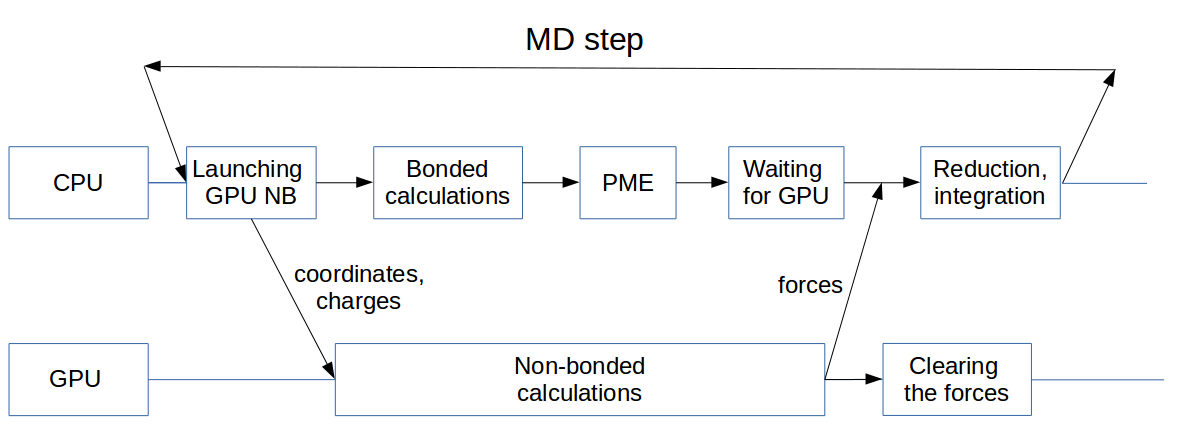
\includegraphics[width=1\textwidth]{pics/mdstep-orig.png}
    \caption{Timeline of MD step in a single-process GROMACS simulation}
    \label{fig:step-orig}
\end{figure}
\FloatBarrier

Some steps, such as  the non-bonded work being split into 2 "local" and "non-local" GPU streams, or inter-process communication, are deliberately omitted from the figure, as they are not the focus of the project. 

% In the case of a certain process doing only the PP or PME work, the corresponding components are not launched. 

%There exist several load balancing mechanisms in GROMACS, which are described below
\section{Load balancing} \label{PMEtuning}
Changing the electrostatic interaction length cut-off, as mentioned in the section \ref{sec_ewald}, influences the amount of computation performed in long- and short-range parts of the MD step. GROMACS uses this fact for the automatic load balancing at the beginning of the simulation run. Periodically the Fourier grid spacing is scaled (the Coulomb cut-off is adjusted accordingly); the average step run-time is measured over the next period. Eventually, the parameter set with the best simulation performance is chosen as the optimal. This allows to increase the utilization of CPUs and GPUs both in single- and multi-process scenarios on a single compute node. 

What is commonly happening with the load balancing is that the relatively small CPU PME work is traded for much larger amount of the GPU NB work (by increasing the grid spacing and the cut-off distance), while benefiting the overall simulation performance \draft{(mention efforts).} This is the case where the GPU PME implementation could possibly alleviate the CPU performance bottleneck. 

\section{Domain decomposition} \label{chapter:DD}
Since most interactions in molecular simulations are local, domain decomposition is a natural way to decompose the system for the multi-node, multi-process simulations. In domain decomposition, a spatial domain is assigned to each process,
which will then integrate the equations of motion for the particles that currently reside in its local
domain.

GROMACS currently uses the eighth shell method, which is described in the GROMACS 4 paper \cite{gromacs4dd}. In the most general case of a triclinic unit cell, the Cartesian space in divided with a 1-, 2-, or 3-D grid in
parallelepipeds which are called domain decomposition cells. Each cell is assigned to a certain particle-particle 
process. 

The multi-process PME calculations can have a separate discrete grid decomposition.
However, since within PME all particles interact with each other, global communication is required (mostly for the FFT and spreading stages). 

The global broadcast communication is usually the limiting factor for scaling. It also introduces the new degree of freedom into already complex task of the empirical load balancing - now the simulation not only depends on the CPU/GPU load, but on the network load as well! 
 To reduce the effect of this problem, some processes are selected to do only the PME calculation, while the other processes, called particle-particle (PP) processes, do the rest of the work - the bonded and non-bonded summation. The number of the PME-only processes is usually limited to $\frac{1}{4}$ of the total process number. When the number of PME processes is reduced by a factor of
4, the number of communication calls is reduced by about a factor of 16. Or put differently, the simulation can now effectively scale to 4 times more processes.
 
\iffalse
Multi-process GROMACS simulations have dynamic load balancing capabilities as well.
The system is partitioned over the processes at the beginning of each MD step in which neighbour
searching is performed.  
When different processes have a different computational load (load imbalance), all processes will have to
wait for the one that takes the most time. One would like to avoid such a situation. Load imbalance
can occur due to three reasons:
\begin{itemize}
\item inhomogeneous particle distribution
\item inhomogeneous interaction cost distribution (e.g. charged/uncharged)
\item statistical fluctuation (only with small particle numbers)
\end{itemize}
That is why there exists a dynamic load balancing algorithm where the volume of each domain decomposition
cell can be adjusted independently.
\fi

\begin{figure}
    \centering
    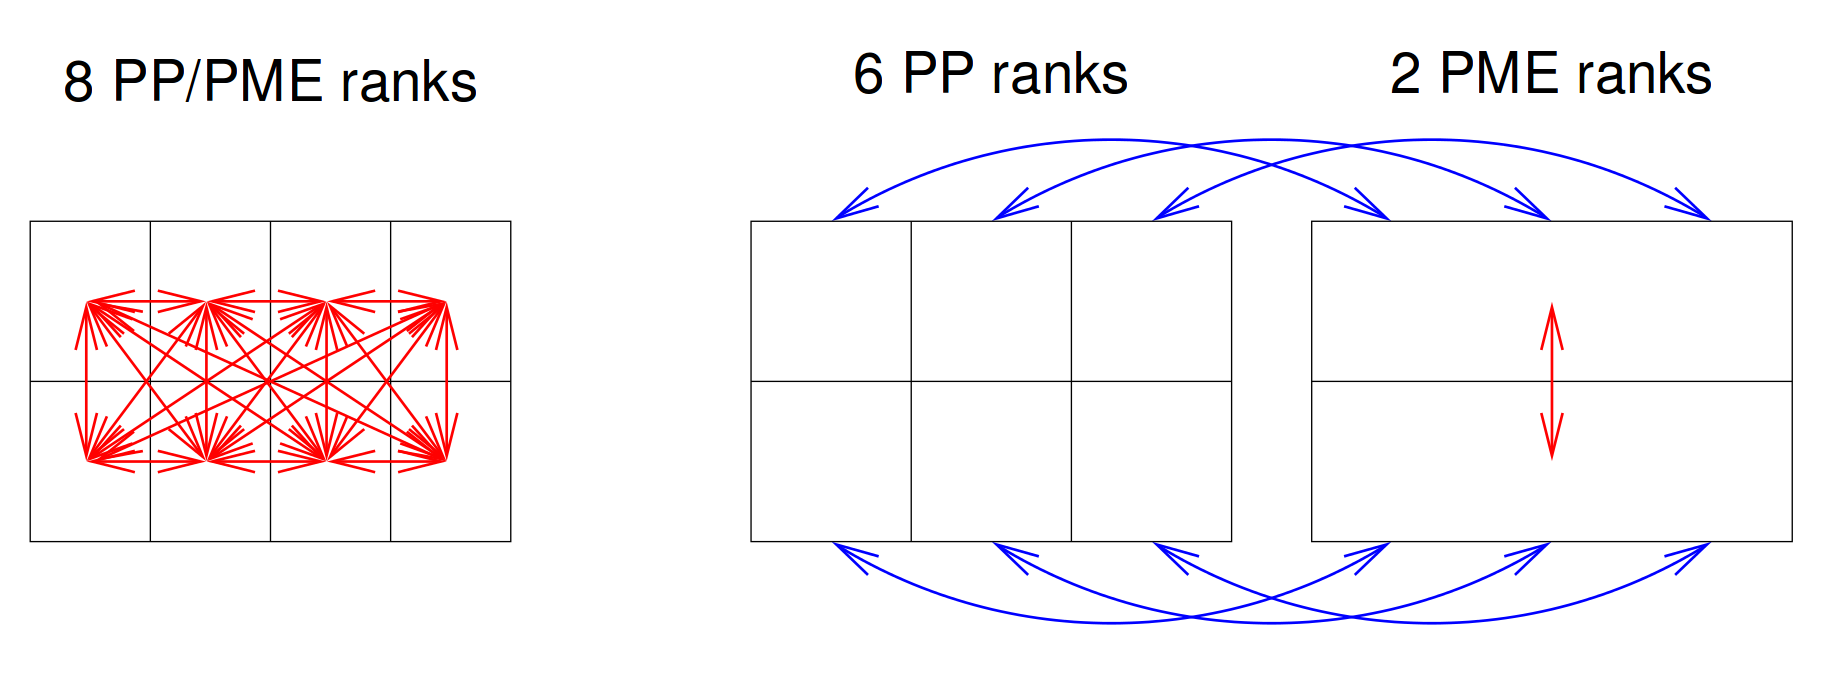
\includegraphics[width=1\textwidth]{pics/DD.png}
    \caption{Example of domain decomposition over 8 processes without (left) and with (right) PME-only processes}
    \label{fig:DD}
\end{figure}
\FloatBarrier

Additional PP - PME coordinate and force communication (blue arrows) is required, but the total communication complexity is lower.

%\draft{no reference to the figure!}

\newpage
\chapter{Implementation of PME on a GPU}

In this chapter, the PME on a GPU implementation details and choices are described.

\section{GPU programming}

General-purpose computing on graphics processing units (GPGPU) is the use of a GPU, which typically handles computation only for computer graphics, to perform computation in applications traditionally handled by the CPU. The main reason for this phenomenon is GPU having a lot of specialized processing units, allowing for efficient SIMD (Single Instruction Multiple Data) approach in algorithms with exposed parallelism and minimum amount of branching.

Currently there are 2 main toolkits for GPU programming: NVIDIA's proprietary platform CUDA, and Apple/Khronos Group's OpenCL standard which is supported by many hardware vendors. While OpenCL aims higher, and unlike CUDA, is targeting not only NVIDIA hardware, and not only GPUs, it has not gained much traction yet. CUDA is a single-vendor platform directly tied onto its implementation; OpenCL is a wider standard which by itself does not guarantee adequate performance on a specific hardware.

Due to reasons described in the project scope section \ref{chapter_scope}, CUDA toolkit (version 7.5) was chosen for the PME implementation. In recent years, several popular MD simulation packages have adopted and explored CUDA implementations of PME: AMBER \cite{amber}, ACEMD \cite{acemd}, LAMMPS \cite{lammps}.

%The CUDA platform is a software layer that gives direct access to the NVIDIA GPU's virtual instruction set and parallel computational elements, for the execution of compute kernels. The CUDA platform is designed to work with programming languages such as C, C++ and Fortran. 

\section{CUDA glossary}
Here is a basic glossary of CUDA terms that are used throughout the report.
 
%some excerpts from a CUDA programming guide to give a basic idea of GPU structure.

Thread - smallest independent sequence of programmed instructions.

Kernel - the function that is being launched on a GPU in many parallel threads.

Stream - sequence (possibly one out of several) of kernels and/or functions being launched on a GPU.

Streaming multiprocessor (SM) - a processing unit handling up to hundreds of threads. A single GPU can have up to dozens of SMs.

Warp - the smallest group of threads executed in parallel by a single SM. Warp size is currently always 32. Individual threads composing a warp start together at the same program address, but they have their own instruction address counter and register state and are therefore free to branch and execute independently (increasing the runtime). The term warp originates from weaving, the first parallel thread technology. 

Block - a group of threads of a constant size. Usually the size is chosen by a programmer as multiple of the warp size. A block is assigned by CUDA runtime to be executed in its entirety by a single SM. For developers convenience, threads within a block can be accessed by 1D, 2D or 3D indices.

Grid - a group of blocks. Grids can also have 1D, 2D or 3D structure - purely for developers convenience.
\begin{figure}
    \centering
    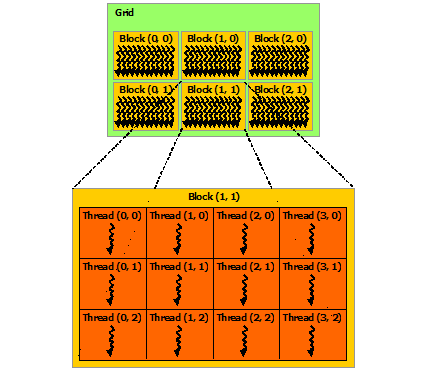
\includegraphics[width=0.7\textwidth]{pics/grid-of-thread-blocks.png}
    \caption{CUDA kernel execution units hierarchy: a grid of blocks of threads}
    \label{fig:grid}
\end{figure}
\FloatBarrier

Global memory - a high-latency memory bank residing on the GPU, which can be accessed by all the kernels simultaneously.

Shared memory - a low-latency memory bank, has a scope of a single kernel's block. It does not retain the information between the kernel launches.

Texture memory - a read only GPU memory bank, optimized for 2D access pattern; uses smaller cache lines with respect to the global memory.

Divergence - the behaviour of the threads in the same warp executing different instructions at the same line of code based on a condition. What is actually happening on GPU SM's is that all the threads have to go through all the branches of a conditional, while the specific threads ignore the instruction result if the condition is false for them. Divergence reduces the kernel performance.

Coalesced memory access - an optimal behaviour for accessing the memory within CUDA device code. The neighbouring threads within a warp have to access the neighbouring 4-byte long memory areas for the best cache utilisation, as data is cached in continuous cache lines (sized 128 bytes). 

%\draft{Should go through all the terms in the text}.

%
%Launch bounds
%Architecture 
%Compute capability 

%sort me

\section{PME GPU scheduling}

The figure \ref{fig:step-gpu} shows the schematic of a modified version of the MD step. Again, just like for the original MD step (figure \ref{fig:step-orig}), multi-process communication details are omitted. 
\begin{figure}[h!]
    \centering
    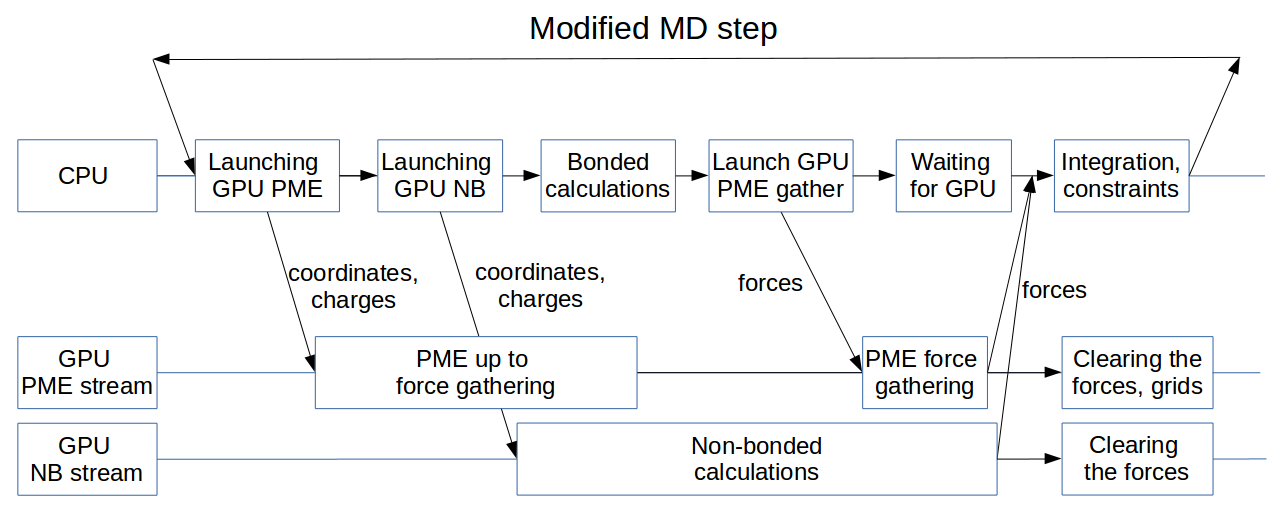
\includegraphics[width=1\textwidth]{pics/mdstep-gpu.png}
    \caption{Timeline of a modified MD step with PME GPU}
    \label{fig:step-gpu}
\end{figure}
\FloatBarrier

The PME computations are scheduled into a separate, high-priority stream of commands.

The reason for PME GPU launch being split into two blocks is that the CPU PME uses the buffer with bonded forces for the calculation.
Therefore, the easiest way of plugging the PME GPU calls into the existing code was to copy the computed bonded forces buffer to the GPU for the reduction in the gather kernel. However, everything before the gathering stage should be launched as soon as possible, even before the non-bonded work.

%MD step modifications are preliminary and might be adjusted in the future, especially for the hypothetical multi-process case.

% The PME GPU stream is also assigned higher priority, in hopes of achieving so called "preemption"

% This split does not appear to critically affect the performance, as the non-bonded GPIU  

% this is a step for PP on the same rank

Implementation of the individual stages of the PME is discussed below.

\section{Sending input data to GPU}
In the beginning of each MD simulation step the particle charges and coordinates are copied to the CUDA device.

Additional input data that is copied to the GPU only occasionally (on any step during which the domain decomposition or configuration can possibly change) includes
\begin{itemize}
\item B-spline moduli for all 3 dimensions;
\item Local grid line indices size of 5 times the grid size to allow for particles (to be out of the triclinic unit-cell by up to 2 box lengths in each direction, which might be required for a very skewed unit-cell)
\item Reciprocal box vectors
\end{itemize}
All of this data is computed on a CPU. It has a low computational effort and parallelization possibility. The grid line indices are just lookup tables for a modulo operation results with some corrections for the rounding issues, and modulo is a rather costly operation on a GPU.

The copying of coordinates and charges constitutes the majority of each step's initial data transfers, because of their regularity (each step) and size (in total 16 bytes per particle with a single precision) as well.

Pairwise particle interaction calculations are also typically performed on GPU in GROMACS, thus in CUDA case the particle data should be shared between the NB (non-bonded) and PME kernels, and only copied once. However, that is not part of the core implementation, as the NB kernel currently use a different particle data layout, so implementing a data reordering kernel would be required. This should not require a lot of effort as it is mostly the question of the higher level MD step code restructuring. It also does not affect the performance adversely, as the data copying operations are overlapped with kernels: by the time the NB particle data transfer starts, the GPU is working on the first PME kernel.

\section{Computation of the spline values and derivatives}
For each particle and for each dimension the individual B-spline interpolation parameters are computed: $l$ values and $l$ derivative values, where $l$ is the spline interpolation order. This naturally suggests using 3 threads per particle. The particle coordinates are used for calculation.
The question of the optimal layout for the spline parameters is interesting. Pictured on \ref{fig:spline} is my choice for an in-memory $\theta$ and $d\theta$ arrays' layout. 
\FloatBarrier
\begin{figure}[h!]
    \centering
    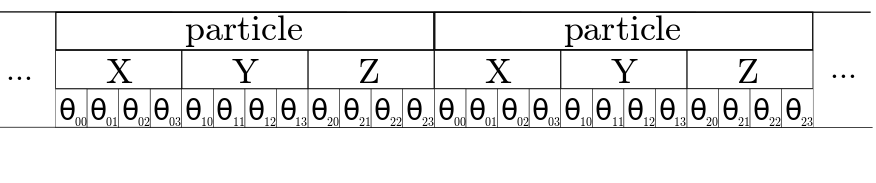
\includegraphics[width=1\textwidth]{pics/theta.png}
    \caption{Data layout for particles' spline parameters}
    \label{fig:spline}
\end{figure}
\FloatBarrier
The reasoning is as follows:
\begin{itemize}
\item The data layout has to be clearly separable into batches for fixed number of particles, for the workload to have a future-proof possibility of batching if needed.
\item A single particle's data for all 3 dimensions has to be kept together for optimizing cache access - the spreading and gathering individual threads are always going to access spline parameters for all 3 dimensions to some extent. 
%\draft{as of now, for order of 4 all the block data makes up 1 (2?) cache line.} 
\item Reads and writes have to be as coalesced as possible.
%\item The possibility of the \draft{global load optimizations} is also open for a single-dimension data.
\end{itemize}

\section{Spreading the particle charges over the grid}
In the first algorithm stage $l^3$ charge contributions to the discrete real-space grid are computed for each particle. The charges, the spline data and the grid-line indices from the previous stage are used.
This could expose $l^3$ parallel threads per particle. 
I choose to have $l^2$ threads per particle so that each thread works on a single line of $l$ contributions for a particle. Every $l$ threads in a warp can still access every single contribution grid-line (in minor dimension) in a coalesced way, while the parallelism is highly exposed; meanwhile, the number of simultaneous atomic operation clashes in the case of the 2 neighbour particles is reduced. Overall, the balance here is between the parallelism and the global memory throughput (as well as the atomic clash latencies). This might require further profiling for different architectures and hardware.

To save on the global memory read/write operations, both the spline calculation and spreading stages are located in a single kernel. This way, the grid-line indices and spline parameters are stored in a shared memory between stages. At first 3 threads per particle compute spline values and particle grid indices at first, the whole block is synchronized, and then $l^2$ threads per particle calculate the charge contributions and atomically accumulate on the global grid. With the PME order of 4 and block size of 128 threads, that gives us 8 particles per block. A single warp ($8 * 3$ threads) is used for the spline calculation part.



%Spread is a very performance-heavy kernel (it takes about \draft{half of total PME GPU run-time}) which is limited by the performance of global memory and its L2 cache because of the atomic operations \draft{on Kepler}. 

\section{Wrapping the grid}
As the method is dealing with a periodic system, the particle spline contributions that go over the grid boundary are supposed to be wrapped over into the other side.
However, integer division and modulo are highly computationally expensive operations in CUDA. %\draft{explain l}
That is why the grid is allocated with additional $(l-1)$ cells in all 3 dimensions. Instead of having modulo operations for grid indices in the spreading, 
a separate wrapping kernel is scheduled afterwards. The kernel only has to atomically add each overlapped grid cell's value to its wrapped address once. A single value is a work of a single thread.

%Each thread works on one overlapped cell, so the number of threads to $(K_1 + l) \cdot (ny + l) \cdot (nz + l) - nx \cdot ny \cdot nz = l \cdot (nx \cdot ny + ny \cdot nz + nx \cdot nz + nx + ny + nz + 1)$ threads. 
%As the kernel runtime is relatively short, it could probably benefit from further optimization using
%The 4-value global load could be definitely exploited...\\
Note that when this GPU implementation will be adapted for the multi-process GROMACS, the wrapping kernel will have to be modified. Only the wrapping in the continuous dimension will be needed; the overlap zones in the decomposed dimensions will have to be communicated between the PME processes, just like it is done in the CPU PME implementation. 

\section{3D FFT} \label{FFTimpl}

Before and after the convolution kernel there is a 3D FFT of the grid to be performed - real-to-complex and complex-to-real, respectively. 
CUDA platform has a cuFFT library which focuses on FFT on a GPU. 
As the scope of the project was the implementation for a single GPU, the implementation required only a single cuFFT function call for a full 3D transform for both directions. 
%However, this function call spawns around 8 different CUDA kernels nonetheless. The kernels being used, and their number depend on the size of the grid, as well as the overlaps. 
Typically for FFT implementations, algorithms are optimized for grid sizes which are multiples of certain small factors (such as 2, 3, 5, 7); it is also recommended to stay away from the large prime factors \cite{cufft}.
With this implementation being a first step of the multi-process PME GPU implementation, the option to use the CPU FFT implementation is provided. The reason is that the FFT stage is responsible for most of communication in the multi-process case, having 2 all-to-all broadcastst between the PME processes. However, using the CPU FFT implementation means that the grid has to be transferred between host and GPU just for these stages, which incurs additional synchronisation latencies.

\iffalse
The cuFFT is not even that much faster than FFTW (single process NUMBERS). 
\fi 
% In the future, some FFT grid size tuning is in order - again, been done on CPU.

% Both directions take similar amount of time (numbers) for the same grid size. 


\section{Reciprocal convolution, energy calculation}

%reference

The algorithm needs to modify each value of the Fourier space complex grid, as well as compute the reciprocal energy and the virial contribution. This kernel only takes about \draft{1\%} of the total run-time, and additionally is embarrassingly parallel. The only common data is the B-spline moduli for all 3 dimensions, read through the texture memory, and the resulting global memory energy and $3 \times 3$ pressure virial (represented by 6 values because it is symmetric). The energy and the pressure virial are reduced block-wise in the shared memory, and then the result is atomically added to the global memory.

Each grid cell is processed by a single thread; for convenience, the block size is rounded to multiples of the minor dimension grid-line size. 
% \draft{This kernel is compute-bound or smem bpound?}

\section{Unwrapping the grid}
After the grid is modified, and complex-to-real FFT is performed, the long-range force contributions are calculated.

For the same reason the Cartesian space grid is wrapped around after the spreading, it gets unwrapped before the force gathering. This does not require atomic operations, as it is only a memory copy operation. Again, a single cell is processed by a single thread. This kernel could be partially replaced by bulk memory copying. 

\section{Force calculation}
Force contribution gathering is a logical counterpart to the charge spreading. The values of the same grid cells affected by charge spreading are now summed up to get the long-range force contribution for the corresponding particles.
The same data layout is used for the spline parameters and indices as well.

%In this kernel, the shuffle reduction was used for compute capability >= 3.0
%\draft{texture objects}

\section{Receiving the results from the GPU}
The computed forces and energy are asynchronously copied back after the respective kernels are done. This means that at the time when the results are needed in the host CPU code, it is enough just to put the synchronisation call which waits for the completion of the asynchronous memory transfers from device to host.

Again, due to the overlap between the NB and PME computation, the transferring of 2 separate resulting force buffers from GPU memory to RAM is not crucial for performance, as only the last transfer happens with the GPU already idle. The OpenMP reduction can then be performed.
%\draft{picture of overlap}

\newpage
\chapter{Results}

In this chapter the PME GPU implementation behaviour and performance is analysed.
\iffalse
The GPUs used for the analysis are build on NVIDIA architectures Kepler and Maxwell.
\fi

\section{Correctness}
The correctness of the GPU PME implementation has been verified by comparing the results with the results of the CPU PME running with the same input data as the reference.
The CPU and GPU PME comparisons were as follows:
\begin{itemize}
\item All of the PME's immediate results such as reciprocal energy, virial and forces have been compared after a single MD step. The relative difference of the reciprocal energy has been no more than $10^{-5}$. 
%This is comparable to the single precision floating point machine epsilon $1.19\times10^{-7}$ being reduced over $10^5$ --- $10^6$ complex grid cells.

%\draft{The interesting part was how given the same input real grid data, the CPU FFT call (using the FFTW library \draft{link here?}) and the GPU FFT call (using the CUDA cuFFT library) produced rather different results. Only the values above certain fixed threshold were the same up to machine precision between the grids.} 

\item All the simulations have been run for 1000 time steps, and the resulting total conserved energy of the system has been compared. It differed by a relative difference on the order of $10^{-4}$, which is within the acceptable fluctuation bounds during the simulation.
 %\draft{(source?)}.
\end{itemize} 

\section{Factors influencing performance}
%\draft{There is a clear division in the PME stages computational effort: computational effort of spreading and gathering (the first and last stages) is dependent on the number of particles $N$ as well as the interpolation order $l$ : $O(N\cdot l^3)$. The effort for the rest of the stages (forward FFT, convolution, backward FFT) is entirely dependent only on the dimensions of the discrete Fourier grid in the single process case. - wtf, its actually NlogN}
%\draft{In multiprocess simulations each 3D FFT execution would require 2 MPI all-to-all communications, where the message size is also dependent on the grid dimensions. However, the communication latency and synchronisation overhead would also be just an important factors.
%As for the single process implementation,} 

%!!! \draft{grid spacing and particles/gridpoint; water represents typical charge density}


The important input parameters affecting the PME performance are the number of particles and the spline interpolation order.
The interpolation order is fixed in this implementation at 4, one of the most common values.

% \draft{The reasons for that...}.

There is also a discrete grid size, which directly affects the runtime of the FFT and convolution stages of the algorithm. However, as it is explained in the section \ref{PMEtuning}, the grid size and spacing can be automatically tuned for better PP/PME load balance, and this is the default behaviour of GROMACS. 

%The average GPU and CPU runtime per single PME step are being compared. The CPU time is measured by standard wallclock functions. The GPU time is taken as a sum of PME kernels' execution times, measured with the use of CUDA events mechanism. \draft{It is shown further that it is hopeless for multiple streams}. The data transfers between the GPU and the host at the step beginning and end are excluded as they are not \draft{significant and in the future will } also beshared with the non-bonded work.



%\section{FFT grid size}

%A system with varying number of particles is ran for several fixed values of the Fourier grid sizes.

\section{Individual kernels performance} \label{chapter_kernels}

The first interesting thing to try is to measure the performance of the individual algorithm components across the different input data sizes.
For this purpose, the kernel performance has been measured using the NVIDIA CUDA profiling tools (\textit{nvprof}, \textit{nvvp}). A synthetic benchmark consisting of water molecules with number of atoms varying from 960 to 1536000 has been used. 
Concurrent kernel execution was turned off to produce more reliable results (the concurrent execution can increase the kernel run times, also increasing the  dispersion). The performance has been measured only for the MD steps after the load balancing, using the GROMACS command-line option "-resetstep". 
 
This data has been measured on the NVIDIA GTX TITAN X GPU, one of the fastest consumer-grade GPUs.

Most of the stages presented at the figure \ref{fig:kernels} correspond to single CUDA kernels. Notable exception is FFT performed by the CUDA cuFFT library, which while having only 2 function calls (real-to-complex and complex-to-real) per MD step, spawns around 8 kernels for each call. The kernels being called also differ depending on the grid size. Moreover, the cuFFT functions have no launch configuration and bounds, unlike CUDA kernels, exposing no granularity control, as they are pre-tuned for optimal performance. 

\iffalse
\begin{figure} [h!]
    \centering
    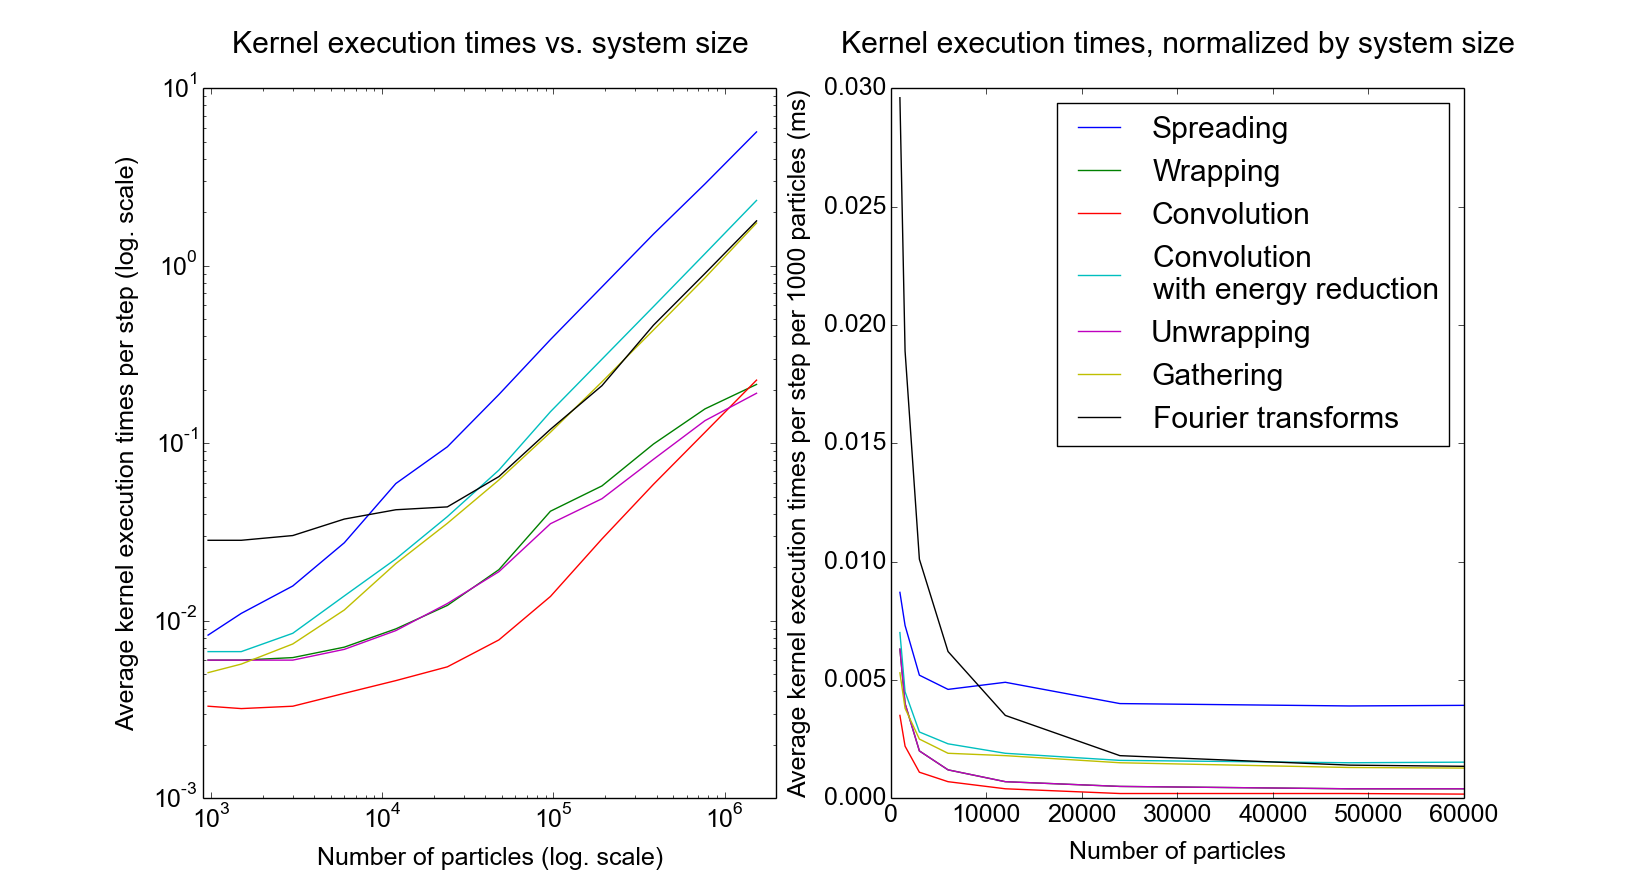
\includegraphics[width=1\textwidth]{pics/kernels-noconcur.png}
    \caption{Performance of the individual PME stages as a function of the number of the input particles on a loglog scale (left) and normalized (right)}
    \label{fig:kernels_}
\end{figure}
\fi
\begin{figure} [h!]
    \centering
    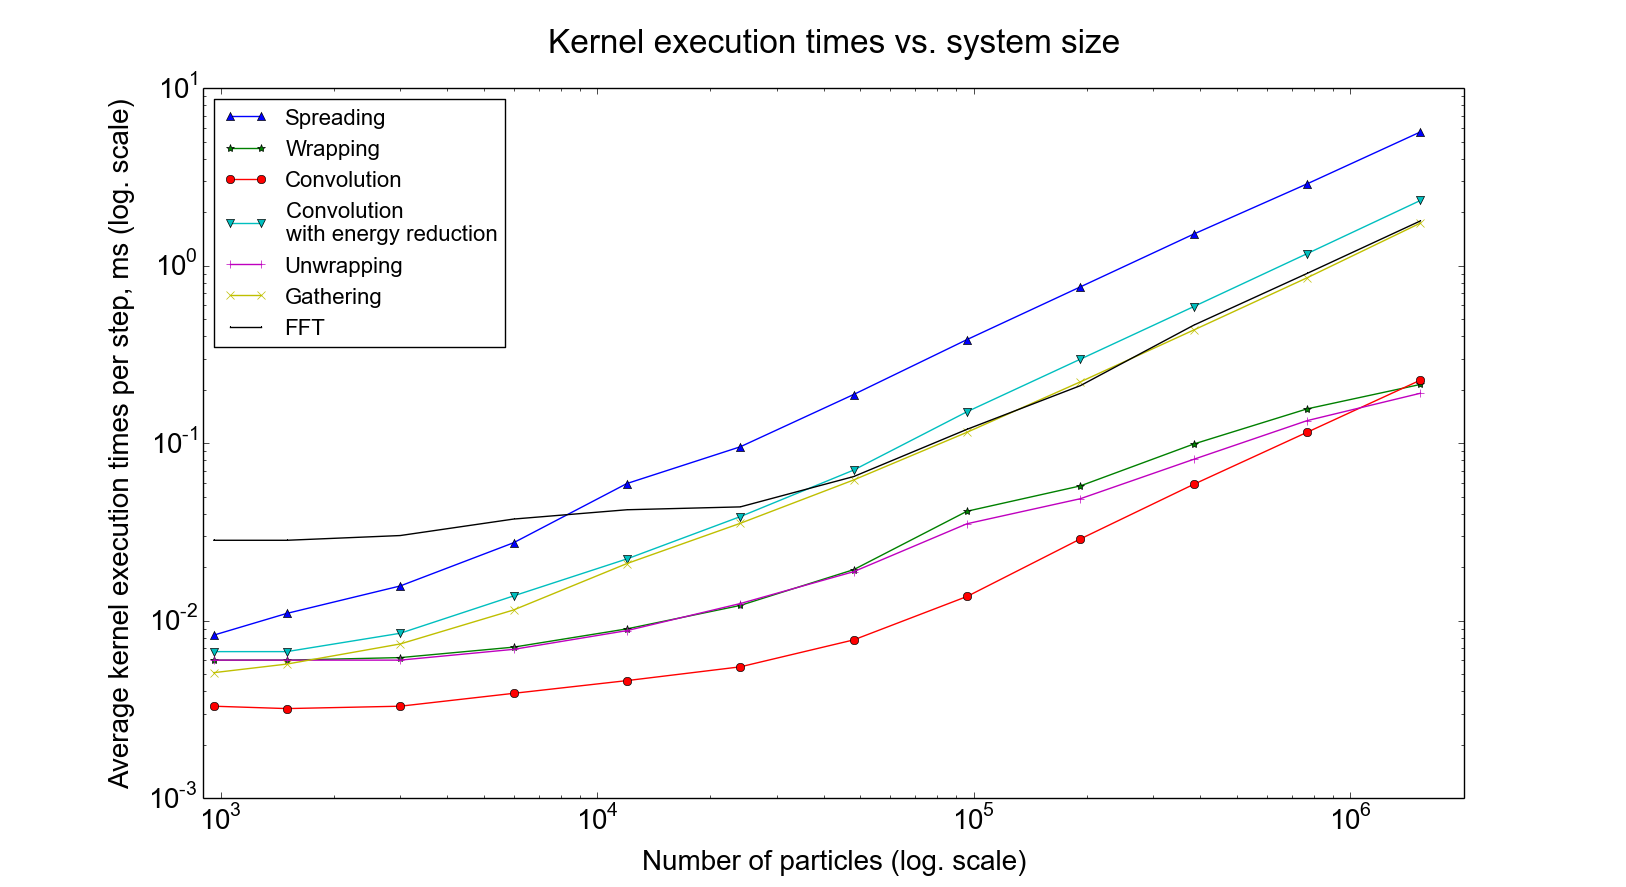
\includegraphics[width=1\textwidth]{pics/kernels-noconcur-2.png}
    \caption{Performance of the individual PME stages as a function of the number of the input particles on a loglog scale}
    \label{fig:kernels}
\end{figure}
% GAPS irrelevant!

It is no surprise overall that the FFT takes the larger ratio of the total GPU runtime, as the input size decreases. The reason for that is that the Coulomb cut-off has a fixed tuning range.
% proofs

Another observable feature on the chart is the wrapping, unwrapping, and the convolution kernels not scaling down well with input sizes. It is also related to their workload being entirely dependent on the grid dimensions.

Finally, it shows that the biggest part of computational time is spent in the spreading kernel. On weaker GPU's (especially with Kepler architecture) this kernel's major bottleneck is the global memory/L2 cache throughput. Atomic operations are the obvious reason for that. Typically the counterpart force gathering kernels is from 2 to 4 times as fast as the spreading. 

\FloatBarrier
\section{Overlapping with the non-bonded kernels}\label{overlapped}

GROMACS uses GPU for the computation of short-range non-bonded electrostatic interactions. One of the project's goals was to study the possibility of calculating both short-range and long-range interactions on the same GPU at the same time, with so called overlapping. CUDA architectures allow for several command streams to execute concurrently, and newer architectures expose 2 possible values of stream priorities.

The modified MD step in this implementation launches the largest chunk of the PME work on a GPU before the NB work is launched (figure \ref{fig:step-gpu}). The PME stream is set to a high priority, using the CUDA runtime API, while the NB stream has lower priority. 
The idea was to have the PME launched in advance and be computed in background, while the NB kernel with its irregular occupancy performs the main computational workload.

Pictured at the figure \ref{fig:overlap} is a typical GPU PME and NB overlap timeline produced in the NVIDIA Visual Profiler with the concurrent kernel execution enabled.
%, on a NVIDIA GTX 750 GPU (Maxwell architecture). 
The top timeline corresponds to the low-priority local NB command stream, the bottom one - to the high priority PME stream. The individual colored bars correspond to kernels (or sometimes memory transfers). 

\FloatBarrier
\begin{figure} [h!]
    \centering
    
\includegraphics[width=1\textwidth]{pics/overlap-crop.png}
    \caption{A concurrent PME/NB kernel execution timeline in NVIDIA Visual Profiler, showing the scheduling problems}
    \label{fig:overlap}
\end{figure}
\FloatBarrier

From the figure it is quite clear that once the low-priority NB work occupies the GPU, the high priority PME kernels have a hard time getting launched as evidenced by the gaps, even though the PME has been launched in advance before the NB kernel has even started. The cuFFT consisting of many kernels amplifies the problem. The gaps are also rather irregular. This counter-intuitive behaviour is obviously related to the GPU internal scheduling mechanism, which NVIDIA does not disclose. 

The only feasible solutions for decreasing the gaps are increasing the granularity of work (launching multiple NB kernels with small batches of data), and ultimately moving to persistent kernels, which are always running on a GPU and routinely polling host-mapped memory for a new workload. This requires a certain amount of effort, of course. Another thing that would help would be the ability to semi-statically delimit the GPU to only allow running certain streams on certain number of SMs. However, such thing currently does not exist in CUDA, and likely will not be exposed in the future.

 What is also happening in the concurrent execution case is that the kernels tend to execute longer. We can take the data from the previous section, run the measurements again with the concurrent kernel execution enabled, and compare the total kernel runtime (table \ref{concur}). Only the small systems avoid this, but the big point of using the GPU parallelization in the first place is that we are able to process robustly much more data in parallel, as compared to the CPU version. 
 
\begin{table} 
\resizebox{\textwidth}{!}{
\begin{tabular} {|c|c|c|c|}
\hline
Number of atoms & 	Kernel runtime,

 sec	& Concurrent kernel 
 runtime, sec	 & Slowdown due to concurrency, \% \\
\hline
960	 & 0.0638&	0.0473&	-25.86\\
1500	& 0.067	&0.051	&-23.88\\
3000	& 0.0773&	0.0624&	-19.28\\
6000	&0.1081&	0.1037	&-4.07\\
12000&	0.1672&	0.1913&	14.41\\
24000&	0.2435&	0.2767&	13.63\\
48000&	0.4319&	0.5306&	22.85\\
96000&	0.8596&	1.3012&	51.37\\
192000&	1.6258&	2.5792&	58.64\\
384000&	3.2326&	4.1111&	27.18\\
768000&	6.2287&	7.5905&	21.86\\
1536000&	12.1713&	13.1279&	7.86\\
\hline
\end{tabular}
}
\caption{Comparison of concurrent and non-concurrent PME GPU kernel runtime}
\label{concur}
\end{table}

\FloatBarrier

\iffalse
\begin{table}
\resizebox{\textwidth}{!}{
\begin{tabular} {| l | c|c|c|c|c|c|c|c|c|c|c| c |}
\hline
Number of particles, thousands & 0.96 & 1.5 & 3 & 6 & 12 & 24 & 48 & 96 & 192 & 384 & 768 & 1536 \\
\hline
Kernel runtime, sec&	0.0638	&0.067	&0.0773	&0.1081	&0.1672	&0.2435&	0.4319&0.8596&	1.6258	&3.2326&	6.2287&	12.1713 \\
\hline
Concurrent kernel runtime, sec&	0.0473&	0.051&	0.0624	&0.1037 &	0.1913	&0.2767&	0.5306	&1.3012	&2.5792	&4.1111&7.5905&	13.1279 \\
\hline
Kernel concurrency slowdown, \% & -25.8 &-23.88 & -19.28& -4.07 & 14.41 & 13.63 & 22.85 & 51.37 & 58.64 & 27.18 & 21.86 & 7.86 \\
\hline
\end{tabular}
}
\caption{The comparison of concurrent and non-concurrent PME GPU kernel runtime}
\label{concur}
\end{table}
\FloatBarrier

\fi

%Overall, this result is somewhat disappointing, and that is even before the kernel launch overhead and memory transfer overhead are taken into account.


\section{CPU and GPU performance comparison}

For the multi-process simulations it is sensible to compare the overall simulation performance results by the single characteristic the end user is most interested in - the simulation time computed per real time. In GROMACS, it is usually measured in ns/day - amount of nanoseconds of the simulation runtime per real wall-clock time elapsed for computation.

The input data used for comparison is a model of ADH enzyme in water, consisting of 134201 atoms.

The simulation is first ran with simulation consisting of 1 PP/PME process. The short-range computations are performed on the high-end NVIDIA GPU GTX TITAN X.    
The PME part is computed in one case on the same GPU, and in another case on the CPU (Intel Core i7-5960X). The number of the OpenMP threads used by the process is varied from 1 to 8.
 
The resulting simulation performance comparison between the CPU and GPU PME is presented at the figure \ref{fig:sepGPUold}.
 
\FloatBarrier
\begin{figure} [h!]
    \centering
    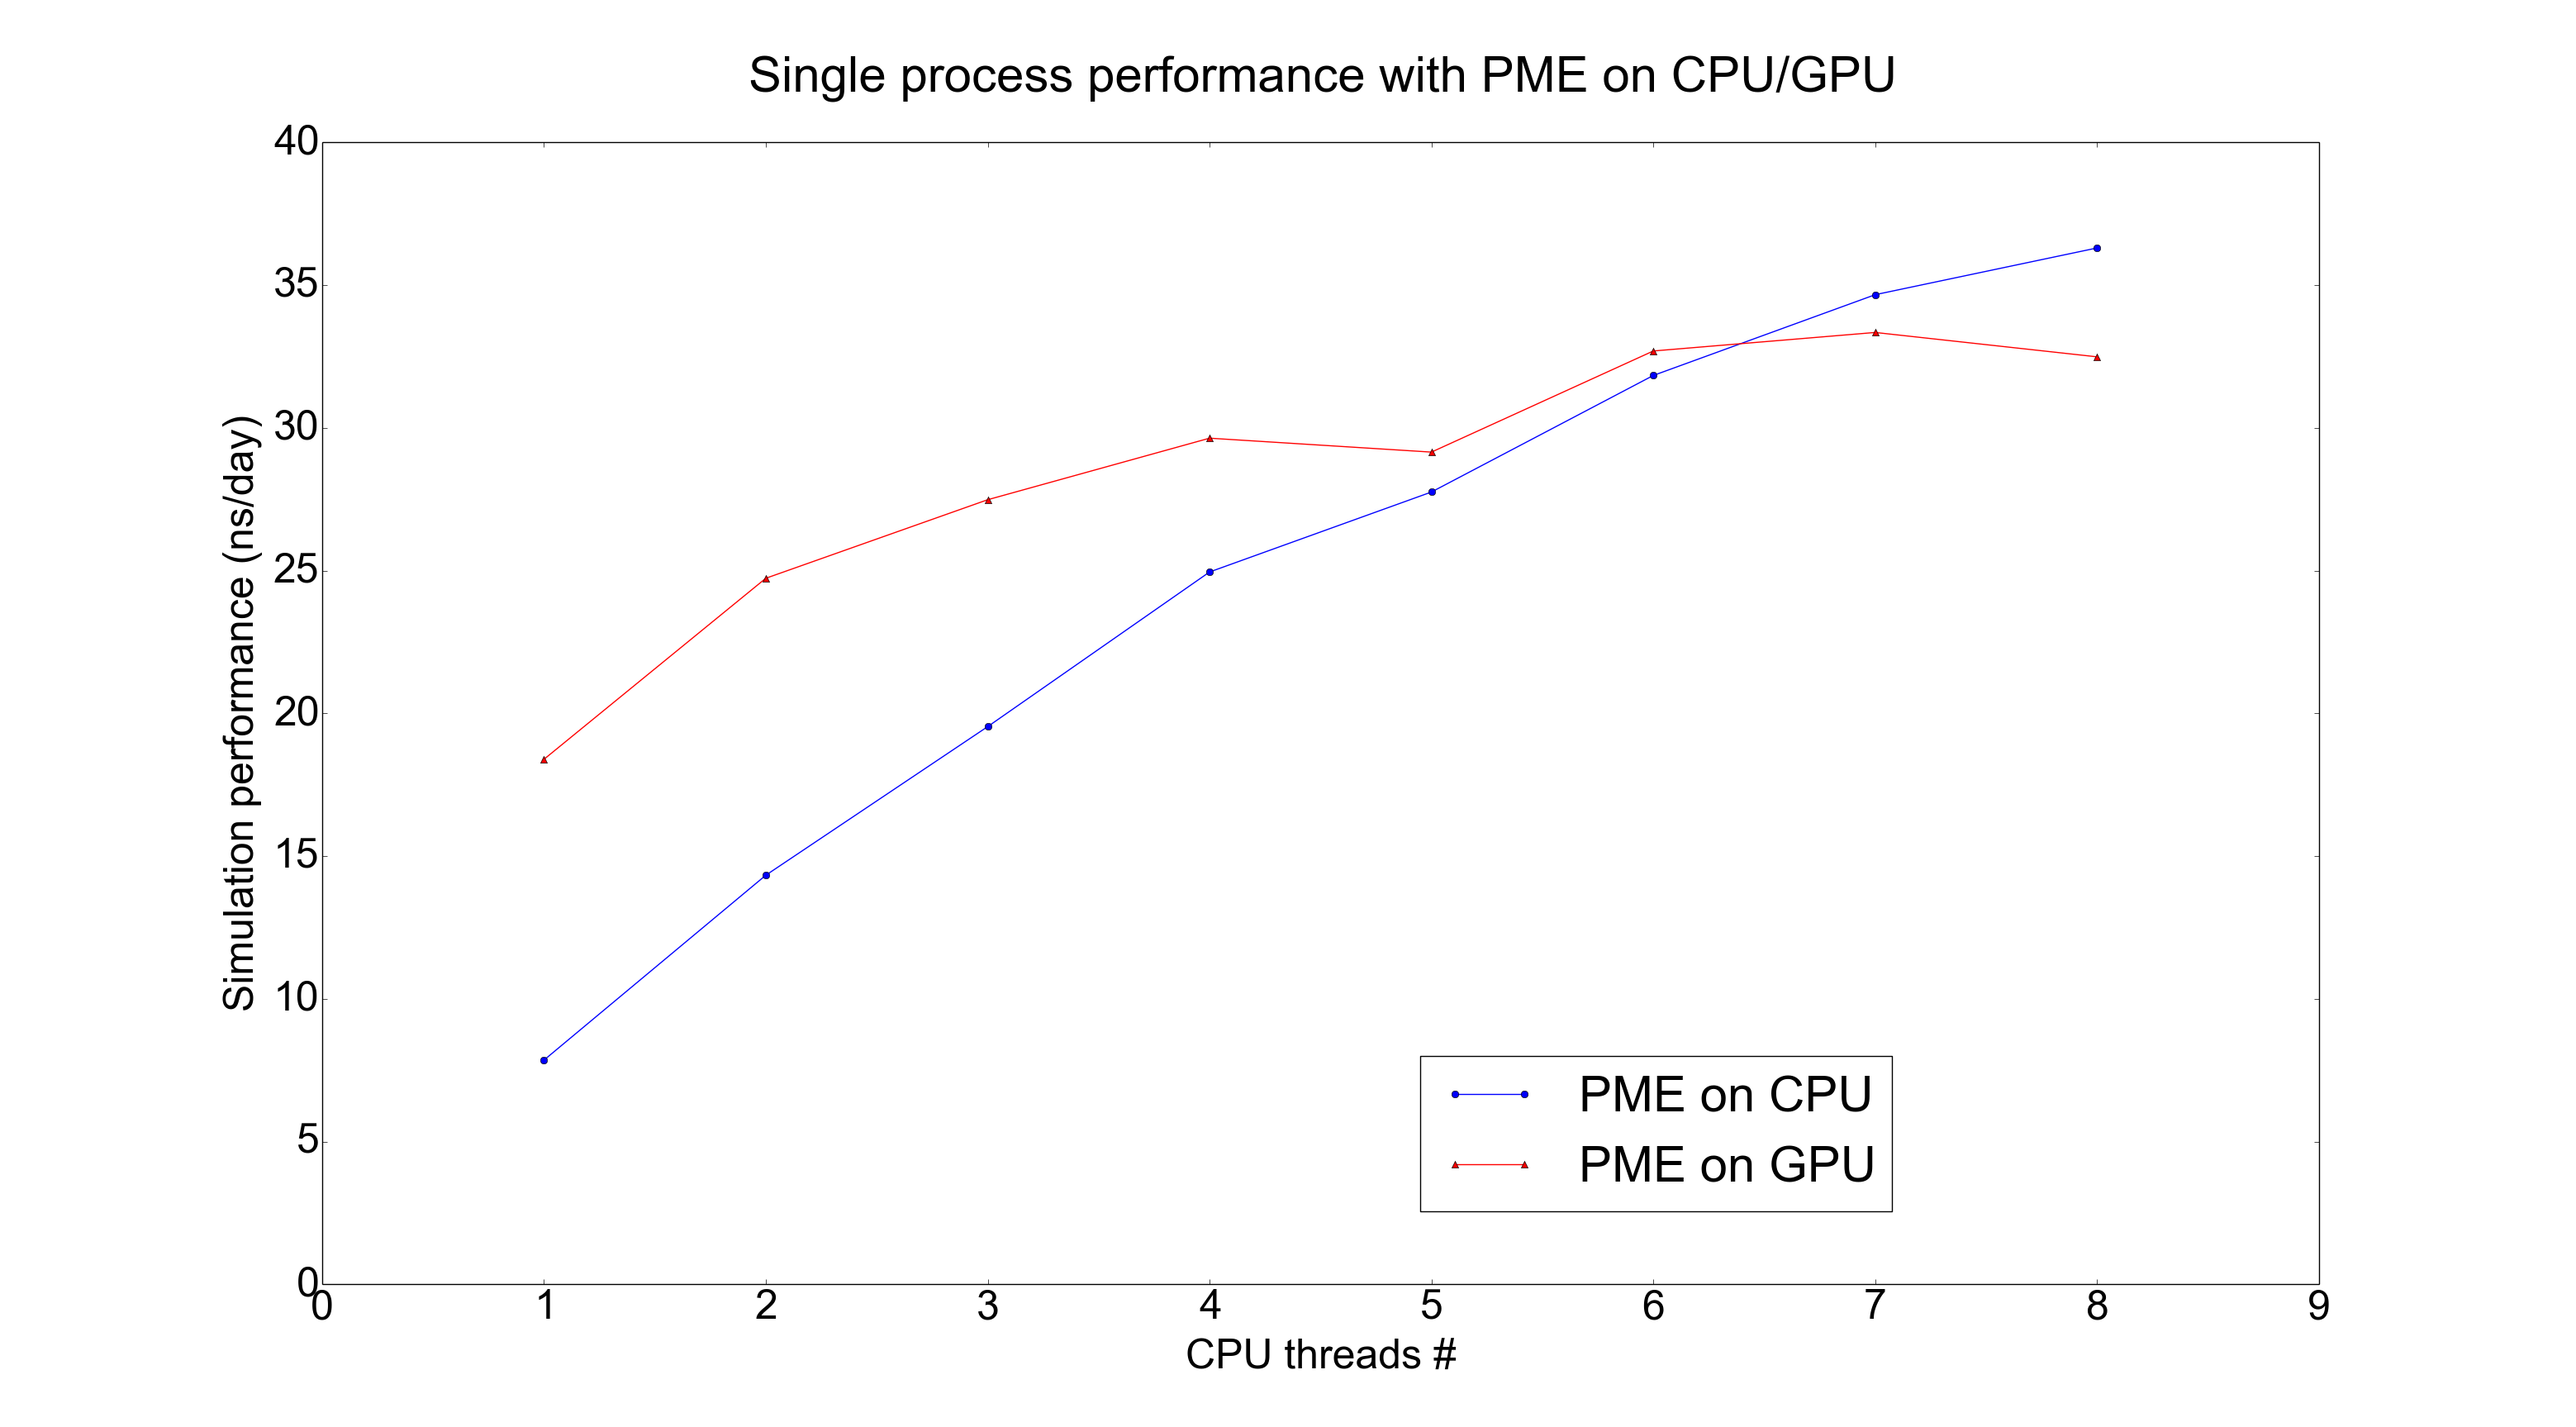
\includegraphics[width=1\textwidth]{pics/CPU_GPU_ADH_SINGLE.png}
    \caption{Simulation performance with a single PP/PME process performing PME on the CPU/GPU}
    \label{fig:sepGPUold}
\end{figure}
\FloatBarrier

The GPU implementation is performing better than a CPU one at a lower number of CPU cores occupied, which makes it viable alternative for machines with strong GPUs and weaker CPUs. 

%{This comparison demonstrates not only a noticeable parallelization speed-up of a separate rank PME on a high-end GPU, but also a possibility of shifting the PME workload onto a GPU from the CPU. It is possible to enhance the load balancing algorithm of GROMACS to perform the switching between GPU and CPU PME dynamically as required.%}

For the next comparison the same machine is used, but a simulation consisting of 2 separate processes is ran: 1 PP and 1 PME process. The PP process performs the short-range computations on the high-end NVIDIA GPU GTX TITAN X, as before.    
The PME process is ran in one case on the CPU (Intel Core i7-5960X), and in another case on the second NVIDIA GPU Quadro M6000. The number of the threads used by the processes is varied from 1 to 8.
 
The resulting simulation performance comparison between the separate CPU and GPU PME ranks is presented at the figure \ref{fig:sepGPUNEW}.
 
\FloatBarrier
\begin{figure} [h!]
    \centering
    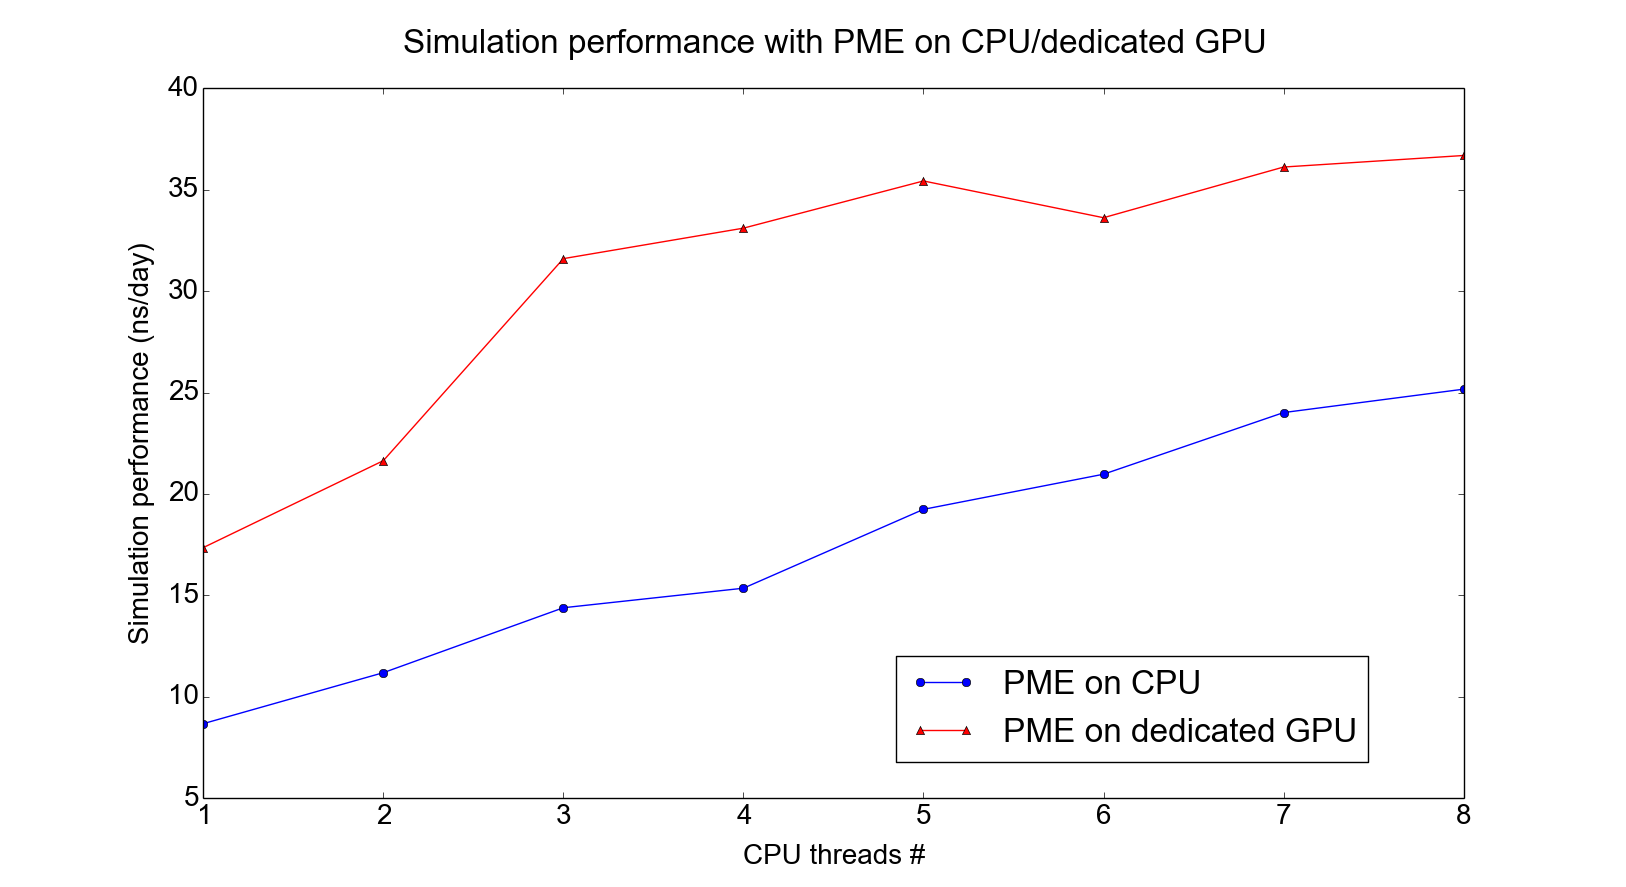
\includegraphics[width=1\textwidth]{pics/CPU_GPU_ADH.png}
    \caption{Simulation performance with a separate PME process working with the CPU/GPU}
    \label{fig:sepGPUNEW}
\end{figure}
\FloatBarrier

This comparison demonstrates not only a noticeable parallelization speed-up of PME on a dedicated high-end GPU, but also a possibility of offloading the PME workload onto a GPU from the CPU. This means making the better use of the machines with abundant GPU hardware, avoiding the CPU bottleneck. It is possible to enhance the load balancing algorithm of GROMACS to perform the switching between GPU and CPU PME dynamically as required.

%\draft{The certain NVIDIA hardware also exposes 2 levels of priorities for CUDA streams. For example, GROMACS running with multiple processes and domain decomposition uses the high priority stream to schedule the calculation of the so called "non-local" non-bonded interactions, and schedule the rest in the low priority stream. Non-local particles are the ones in the buffer zones close to the other parts of the decomposed domain, therefore affecting them; the results of their computation have to be communicated among processes as soon as possible for better performance (FIGURE).}

% Performance of all the GPU work suffers by ...\% on average.
 
    
\iffalse

\section{Separate PME process performance}

For this test, a compute node with 2 16-core AMD Opteron CPUs and 2 NVIDIA GTX TITAN GPUs is used.

In the first case, 3 processes are ran: 1 PP process per GPU, and 1 PME process on CPU. In the second case, 2 processes are ran: 1 PP GPU, and 1 PME GPU. The performance is compared by the simulation time per real time result. The result is shown on a figure \ref{fig:sepGPU}.


\FloatBarrier
\begin{figure} [h!]
    \centering
    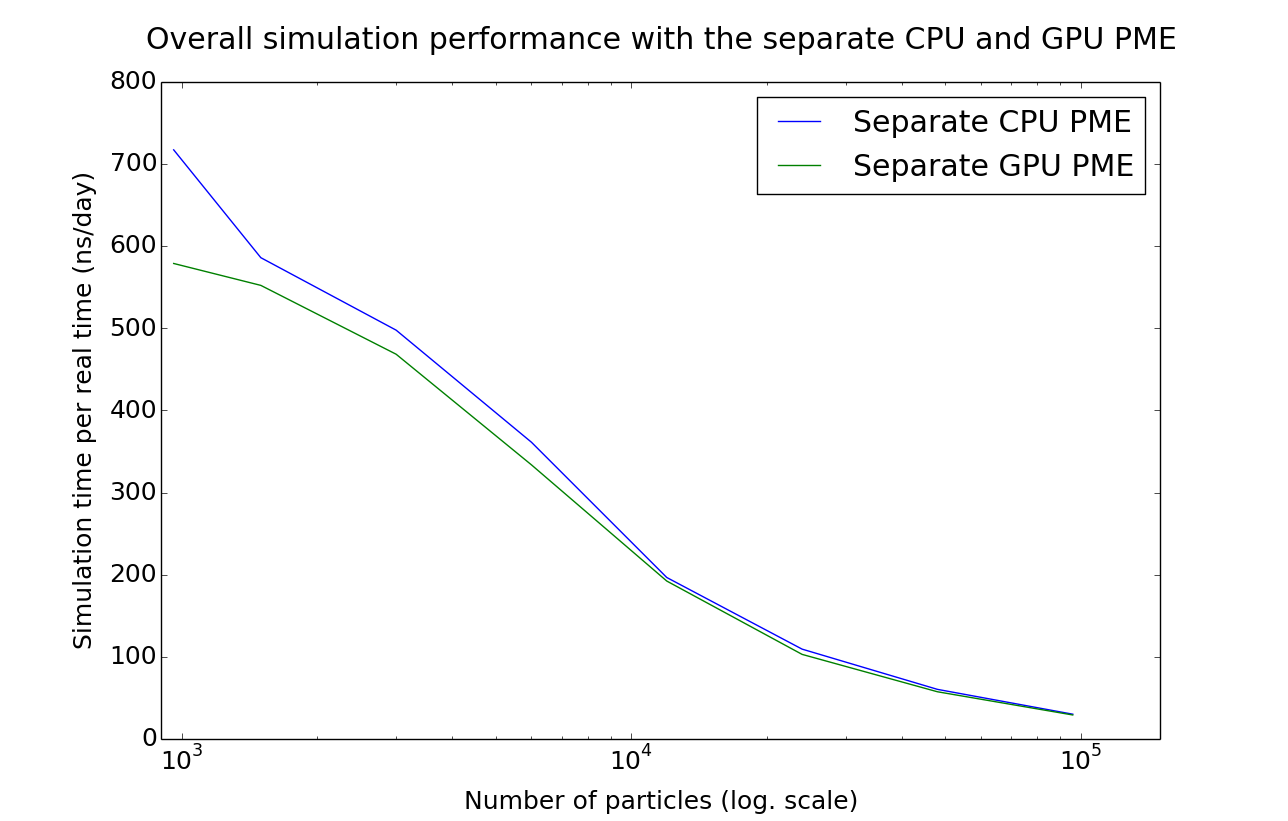
\includegraphics[width=1\textwidth]{pics/GPUCPU.png}
    \caption{Simulation performance with a separate PME CPU/GPU process}
    \label{fig:sepGPU}
\end{figure}
\FloatBarrier

As in the PME GPU case only the listed forces are computed on the CPU (which is a small computational effort), it means that the existence of the PME GPU option now allows for the majority of the simulation workload to be shifted from the CPU to the GPU with non-critical loss in performance. This can potentially mean better GPU performance of GROMACS on the clusters with abundant high-performance GPU hardware, where the bottleneck before would be a CPU PME computation.
\fi

\newpage
\chapter{Conclusions, future work}
This chapter describes the PME GPU implementation current status and its future prospects.

\section{Implementation results}
The PME GPU prototype has been implemented using GROMACS open-source code base within a rather limited scope. 

First and foremost, the GPU PME has only been implemented for a single PME process. This allows it to be ran on a single PP/PME process, or as a single separate PME process interacting with several PP processes. The latter allows a single computer with several NVIDIA GPUs to fully utilize its hardware for the purposes of MD simulations, shifting most of the workload onto GPUs. However, absence of PME decomposition is a barrier to further scaling.

The existing load balancing and tuning mechanisms interact correctly with the PME GPU routines as well. 

Only a single interpolation order (4) is currently supported. There is neither a large effort nor principal obstacles to implementing different orders. 

The FFT stages of the algorithm can be performed either on CPU or on GPU. This leaves a possibility of introducing a multi-process decomposition into PME GPU with minimal effort, reusing the existing communication logic.

The code is expected to be integrated into the GROMACS code base within several months. At the moment of writing it can be accessed at the public Git repository \cite{pmegpugit}.

\section{Multi-process and FFT}

Most stages of the PME algorithm should be trivial to adapt for working only on part of the decomposed grid in the multi-process case.
The main uncertainty for the multi-process GPU implementation of PME is the Fourier transform. One way to go about it would be using the existing CPU FFTW Fourier transform calls with the MPI communication.

Another option would be getting the cuFFT for use with MPI. Techniques for direct GPU-to-GPU communication, like NVIDIA GPUDirect, should definitely be tried in that case.

However, a full 3D Fourier transform on a distributed grid requires 2 all-to-all communications. That would mean at least 6 copy operations of the local part of the grid between the host and the GPU - at least 12 during the single MD step. Such behaviour is rather undesirable, as memory transfers incur additional latencies.
As it has been shown in \ref{chapter_kernels}, even in a single process case better cuFFT performance can be desired.

The question of the efficient communication of the grid data is important for the FFT and the wrapping/spreading stages, doubly so for a GPU.
 
% And then the gather is not that important after all...
\section{PME interpolation order}
The only supported B-spline interpolation order in the current PME GPU implementation is 4. While the commonly used values for the PME interpolation order are 4 and 5, as suggested in \cite{spme}, the value of 4 allows for exactly $32/4^2 = 2$ particles processed by a single warp within spread and gather parts of the algorithm with neither idle threads nor divergence. As 32 is not divisible by 5, with PME interpolation order of 5 those issues will certainly come up.

Continuing this line of thought, interpolation order of 8 might be interesting to try out, as it will eliminate idle threads and divergence as well. The implementation would require only a relatively small effort to adapt to orders other than 4. It would most likely prove useful in a multiprocess case, since increasing the Fourier grid spacing and the interpolation order is a way to decrease the FFT communication requirements.

\section{Scheduling}

As it has been shown in section \ref{overlapped}, scheduling both short- and long-range work on the same GPU within a single process with the ultimate goal of minimizing the critical path runtime is already a problematic task.
There are a few plausible long-term solutions: 
\begin{itemize}
\item Persistent kernels running in the background and polling the host memory for work;
\item Reworking the structure of the program to get away from the strict "one command stream = one part of the algorithm" decomposition logic. Adoption of the more flexible approach: constantly resorting all the PME and NB work chunks into high and low priority streams, using the actual runtime estimates.
\end{itemize}
\iffalse
With the multiprocess and domain decomposition GROMACS is already using the high priority stream to schedule the calculation of the so called "non-local" non-bonded interactions, and scheduling the rest in the low priority stream. Non-local particles are the ones in the buffer zones close to the other parts of the decomposed domain, therefore affecting them; the results of their computation have to be communicated among processes as soon as possible for better performance.
Therefore, in the hypothetical case of the multi-process PME running on GPUs, GROMACS would have to schedule 3 logical GPU streams, and perform the load-balancing for the scheduling order as well.  
\fi
The recommended way of using the current implementation is launching a separate PME process on a dedicated GPU instead of a mixed PP/PME process. This way alleviates the overlapping problems, and also allows for PP decomposition over multiple processes.
%achieved by running the simulation with PME:PP balance auto-tuning.

\iffalse
How are B-spline order	s used?
\fi

\bibliographystyle{plain}
\bibliography{pics/my}

\end{document}